\section{Entwurf des zentralen Systems}\label{l:entwurf}

\begin{figure}[htb]
\begin{center}
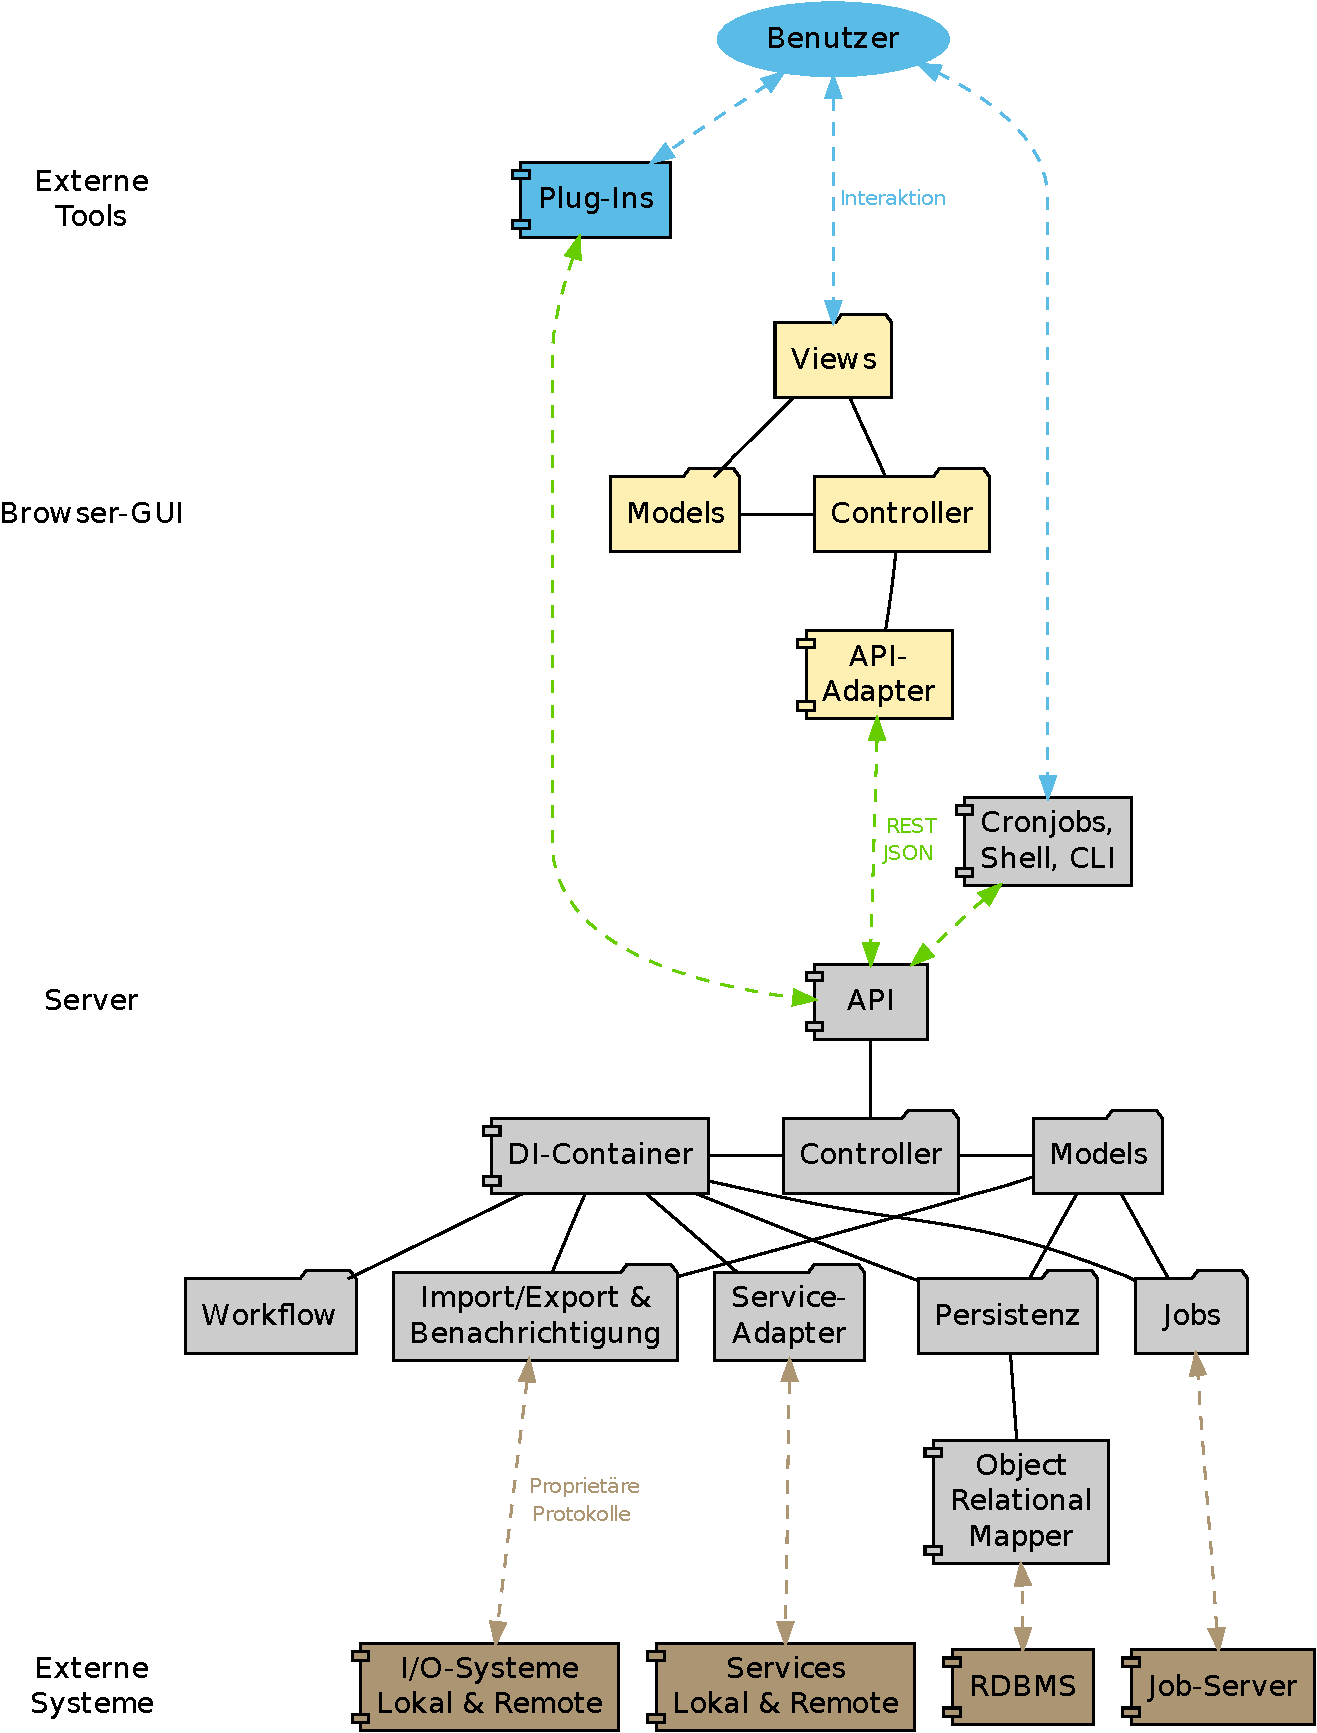
\includegraphics[width=0.75\textwidth]{media/komponenten.pdf}
\end{center}
\caption{Komponententen des zentralen Systems}
\label{chart:komponenten}
\end{figure}

Im vorigen Kapitel \ref{l:konzeption} · S.\pageref{l:konzeption} wurde eine Anwendung konzipiert, die das gesamte Spektrum der Anforderungen abdeckt, die in den vorangegangenen Kapiteln beschrieben wurden. In diesem Kapitel werden die Komponenten beschrieben, die zur Erfüllung der wichtigsten Anforderungen benötigt werden.

Abbildung~\ref{chart:komponenten} liefert einen Überblick über die in den folgenden Abschnitten beschriebenen Komponenten des Systems. \emph{Blau} eingezeichnet sind der Endanwender und externe Benutzer-Werkzeuge wie z.B. Plug-Ins und Software von Drittanbietern. \emph{Gelb} eingezeichnet sind die Komponenten des browserbasierten GUI. \emph{Grau} eingezeichnet sind die Komponenten des Servers. \emph{Braun} eingezeichnet sind (aus Sicht des Servers) externe Dienste, die durch diesen angebunden werden. \emph{Gestrichelte Linien} zeigen Kommunikationsverbindung zwischen Komponenten über Schnittstellen. \emph{Durchgezogene Linien} zeigen Verbindungungen innerhalb eines Systems. 

Der zentrale Bestandteil der Anwendung ist der Server, mit dem verschiedene GUIs über Schnittstellen kommunzieren. Das wichtigsten GUI ist das browserbasierte Interface, da hiermit alle Mitarbeiter arbeiten, dessen Gestaltung in Abschnitt \ref{l:entwurf-gui} · S.\pageref{l:entwurf-gui} und dessen Anbindung an den Anwendungsserver in Abschnitt \ref{l:anbindung-gui} · S.\pageref{l:anbindung-gui} beschrieben wird. Abschnitt \ref{l:entwurf-server} · S.\pageref{l:entwurf-server} beschreibt die Komponenten des Anwendungsserver. 

Zur Validierung des Entwurfes wurde ein Querschnitt durch die vorgestellte Architektur als Prototyp umgesetzt, mit dessen Hilfe sich überprüfen lässt, inwieweit sich das vorgeschlagene Konzept praktisch einsetzen lässt und die entworfene Systemarchitektur geeignet ist, die benötigten Funktionen abzubilden. In Abschnitt \ref{l:implementierung-gui} · S.\pageref{l:implementierung-gui} und \ref{l:implementierung-server} · S.\pageref{l:implementierung-server} wird die prototypische Implementierung der GUI bzw. des Anwendungsservers, die auf dem Entwurf basiert, beschrieben.

Zuerst wird jedoch das Domänenmodell, dass die gemeinsame Grundlage bildet, im nächsten Abschnitt \ref{l:domänenmodell} beschrieben.

\pagebreak

\subsection{Domänenmodell}\label{l:domänenmodell}

\begin{center}
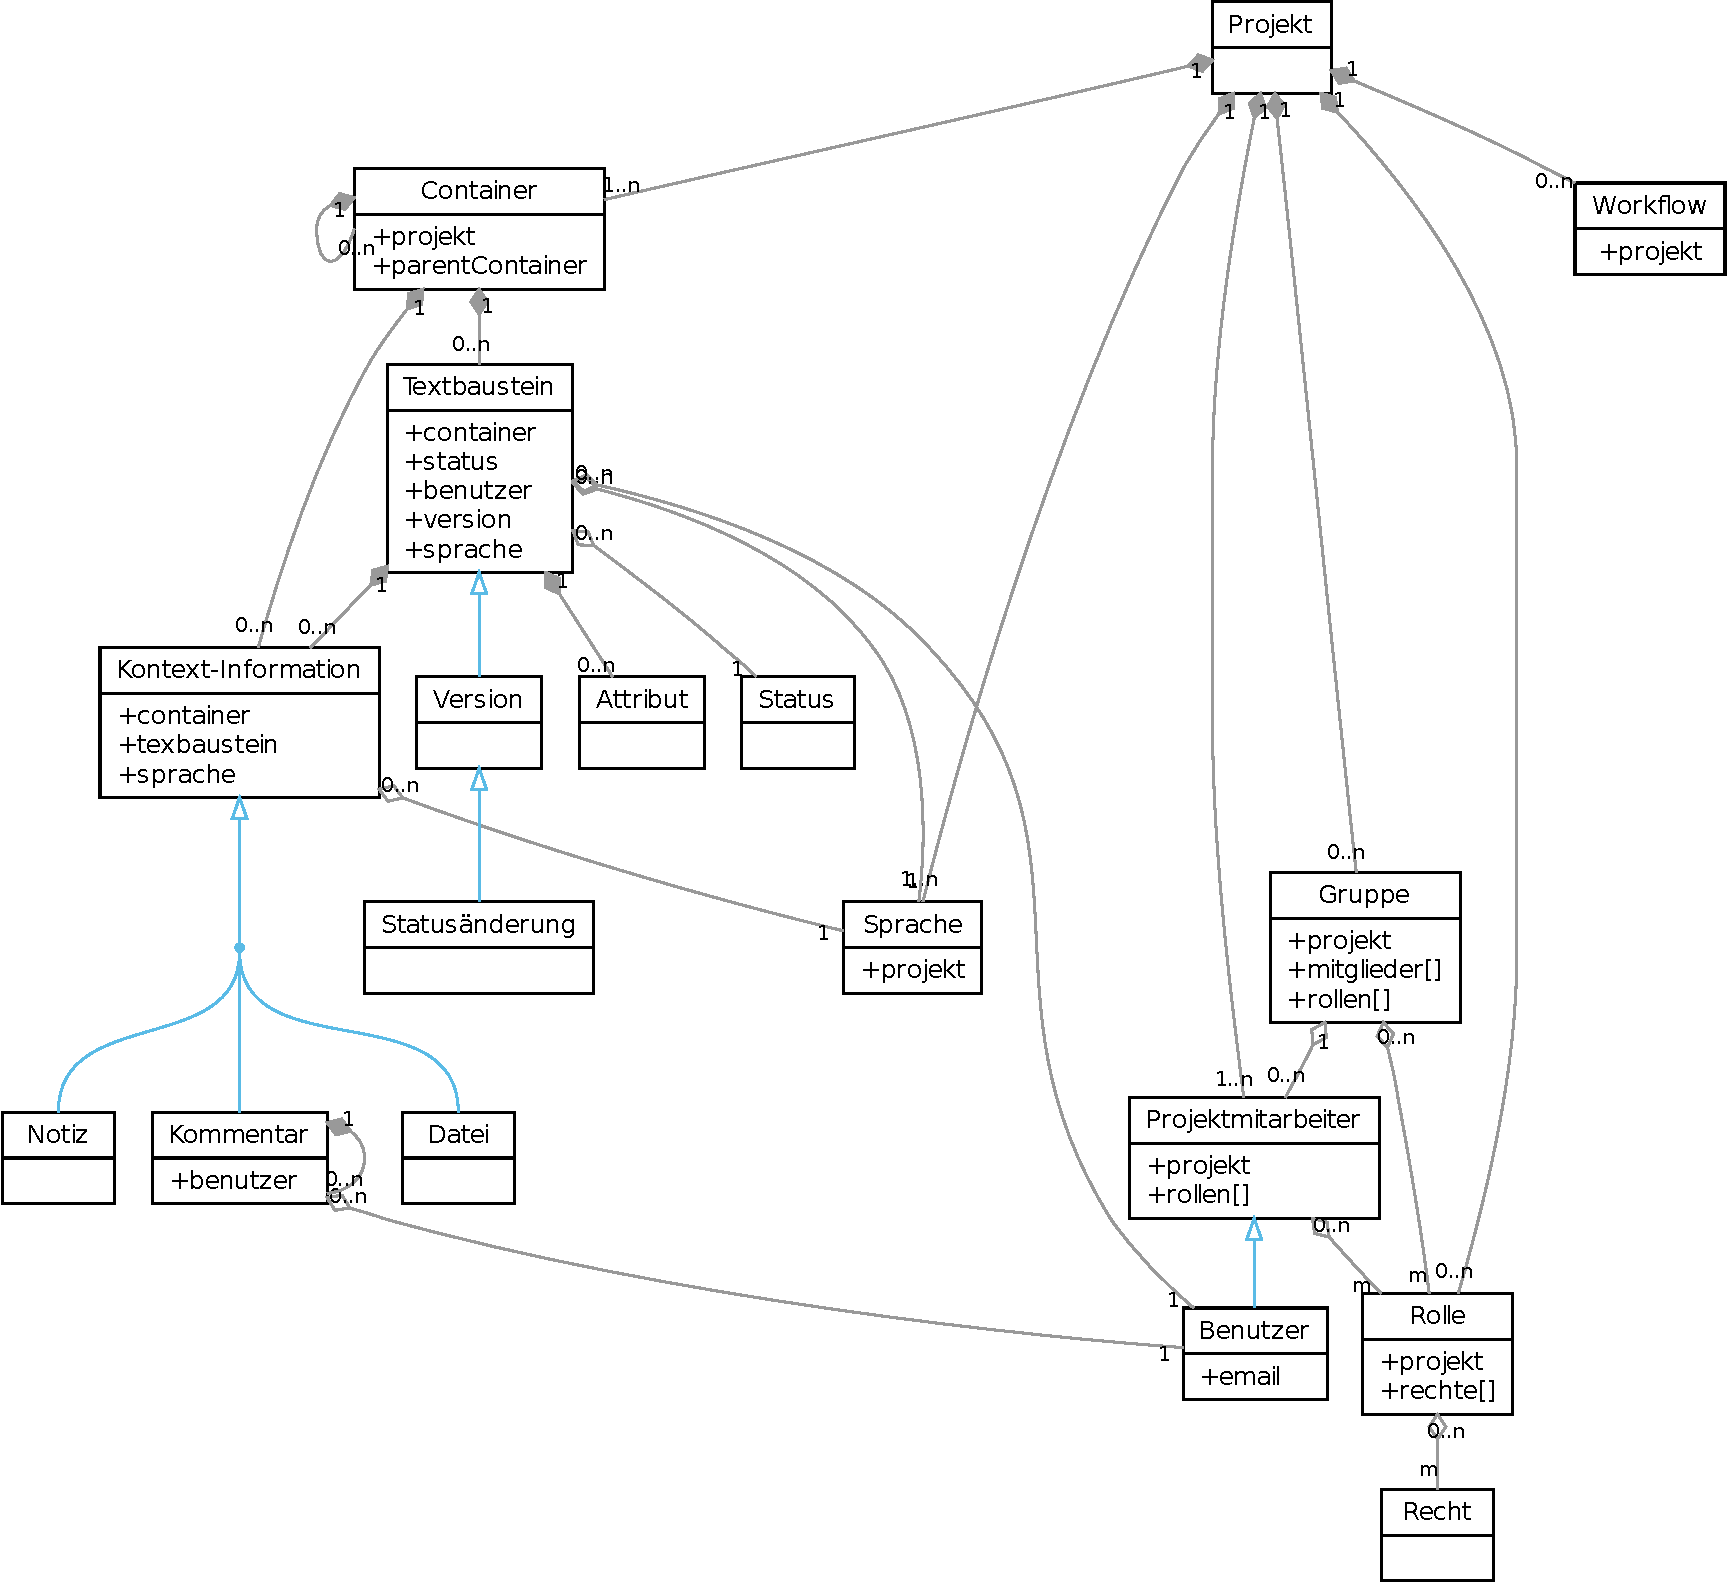
\includegraphics[width=\textwidth]{media/domain.pdf}
\captionof{figure}{Domänenmodell}\label{chart:domain}
\end{center}

Aus den vorangegangenen Überlegungen zur Anwendung und zum Workflow lässt sich ein Domänenmodell extrahieren, die einzelnen logischen Objekte innerhalb der Anwendung beschreibt, mit deren Hilfe alle Operationen abgebildet werden. Abbildung~\ref{chart:domain} zeigt das Modell in der Übersicht, dass die sich im Entwurf der Anwendung in deren Implementierung im Prototyp widerspiegelt.

\textsf{\textbf{Attribut}}\\Beschreibt die Attribute eines Textbausteins.

\textsf{\textbf{Benutzer}}\\Repräsentiert einen Benutzer des Systems

\textsf{\textbf{Container}}\\Containern dienen zur hierarchischen Organisation der Texte innerhalb des Projekts. Containern können weitere Container und Texte enthalten. Eine Container ohne übergeordneten Container befindet sich auf der obersten Ebene. Es kann mehrere Containern auf der obersten Ebene geben.

\textsf{\textbf{Gruppe}}\\Mitarbeiter können in Gruppen zusammengefasst werden. Dies erleichtert die Konfiguration des Workflows und der Rechte.

\textsf{\textbf{Kommentare}}\\Kommentare enthalten Hinweise und Fragen zu einzelnen Texten und Texbausteinen.

\textsf{\textbf{Kontext-Information}}\\Projektspezifische Kontext-Informationen lassen sich hinterlegen und Textbausteinen und Containern zuordnen.

\textsf{\textbf{Projekt}}\\Projekte bildet den Rahmen für alle Texte eines einzelnen Produkts.

\textsf{\textbf{Projektmitarbeiter}}\\Gestattet einem Benutzer die Mitarbeit an einem Projekt und legt dabei fest, welche Rechte dem Benutzer für das Projekt zustehen.

\textsf{\textbf{Recht}}\\Beschreibt ein Recht, eine Operation auf einem Objekt auszuführen.

\textsf{\textbf{Rolle}}\\Beschreibt die verschiedenen Rollen innerhalb der Anwendung. Die Rechte der Rollen sind durch die Zuordnung von Benutzern zu Projekten durch den Projektmitarbeiter immer an das jeweilige Projekt gebunden.

\textsf{\textbf{Sprache}}\\Die Texte jedes Projekts liegen in einer oder mehreren Sprachen vor.

\textsf{\textbf{Status}}\\Beschreibt die verschiedenen Zustände eines Textbausteins (vgl. Abschnitt \ref{l:konzept-workflow-status} · S.\pageref{l:konzept-workflow-status}).

\begin{enumerate}\itemsep -5pt
\item \texttt{Neu}, Textbaustein erzeugt
\item \texttt{Leer}, Textbaustein definiert
\item \texttt{Befüllt}, Textbaustein mit Inhalt befüllt
\item \texttt{Korrigiert}, Orthografie geprüft
\item \texttt{Geprüft}, Inhalt geprüft (Qualitätsicherung)
\item \texttt{Freigegeben}, durch Kunden freigegeben
\item \texttt{Veröffentlicht}, in Produkt übernommen
\end{enumerate}

\textsf{\textbf{Statusänderung}}\\Beschreibt eine Änderung eines Status durch einen Benutzer, z.B. durch Freigabe oder Überprüfung.

\textsf{\textbf{Textbaustein}}\\Beschreibt einen einzelnen Textbaustein.

\textsf{\textbf{Version}}\\Beschreibt eine Version des Inhalts eines Textbausteins.

\textsf{\textbf{Workflow}}\\Beschreibt einen projektspezifischen Workflow.

\pagebreak

\subsection{Entwurf eines browserbasierten GUI}\label{l:entwurf-gui}

Das browserbasierte GUI der Anwendung ist der wichtigste Zugang zum System, da es von allen Mitarbeiter zu irgendeinem Zeitpunkt verwendet wird. Die Zeit, die der Einzelne damit verbringt kann sich je nach Rolle stark unterscheiden. Neben den sehr unterschiedlichen Anforderungen and das GUI sind die Benutzer auch technisch sehr unterschiedlich stark versiert, wie in den Personas in Kapitel \ref{l:personas} · S.\pageref{l:personas} gezeigt wurde. Diesen Umständen muss bei der Gestaltung eines GUI Rechnung getragen werden. In Anlehnung an \cite{nielsen} wurden für den Entwurf der browserbasierten GUI folgende Leitlinien gewählt:

\begin{enumerate}\itemsep -5pt
\item{Das wichtigste zuerst: Die aktuelle Aufgabe soll immer im Fokus der Darstellung liegen.}
\item{Schnell zum Ziel: Alle Aufgaben müssen leicht und umkompliziert durchführbar sein.}
\item{Nicht ablenken: Veränderungen in der Darstellung, z.B. durch Benachrichtigungen, lenken ab und müssen deswegen so gestaltet sein, dass diese sich nach den Präferenzen des Nutzers richten.}
\item{Hilfe nur einen Klick entfernt: Das Hilfesystem muss kontextsensitiv verfügbar sein und ist eine Kernfunktion der Anwendung}
\end{enumerate}

Da die Anwendung von allen Benutzern gerne verwendet werden soll und vor allem die Usability und die Zeitersparnis ein wichtiger Punkt sind, wie man auch skeptische Mitarbeiter überzeugen kann, mit ihren alten Gewohnheiten zu brechen, ist die Beachtung dieser Grundsätze essentiell. Funktionalitäten, die nur von wenigen gebraucht werden, sollten, wenn überhaupt, optional einblendbar sein. Die Konzeption des Systems ermöglicht es leicht, zusätzliche Anwendungen für besondere Benutzergruppen zu schaffen, z.B. Plug-Ins für die speziellen Werkzeuge einzelner Mitarbeiter. Für diese \typoquotes{Power-User} ist dieser Weg meistens der bessere Weg.

\begin{table}
\begin{center}
\begin{tabular}{@{}l c c c c c c c}
& \textbf{Eva} & \textbf{Lotte} & \textbf{Torsten} &  \textbf{Jorinde} & \textbf{Jan} & \textbf{Arthur} & \textbf{Markus}\\
{\small Operation (vgl.~\ref{l:workflow})} & {\small Konz.} & {\small Des.} & {\small Texter} & {\small Übersetz.} & {\small Prod.} & {\small Projektl.} & {\small Kunde}\\
\hline\\[-1.5ex]
Definieren         & \HarveyFull      & \HarveyQuarter   & \HarveyEmpty    & \HarveyEmpty    & \HarveyEmpty   & \HarveyEmpty     & \HarveyEmpty \\
Schreiben          & \HarveyQuarter   & \HarveyEmpty     & \HarveyFull     & \HarveyFull     & \HarveyEmpty   & \HarveyEmpty     & \HarveyEmpty \\
Korrektur          & \HarveyEmpty     & \HarveyEmpty     & \HarveyHalf     & \HarveyHalf     & \HarveyEmpty   & \HarveyQuarter   & \HarveyQuarter \\
Qualitätskontrolle & \HarveyQuarter   & \HarveyEmpty     & \HarveyEmpty    & \HarveyEmpty    & \HarveyEmpty   & \HarveyFull      & \HarveyHalf \\
Freigabe           & \HarveyEmpty     & \HarveyEmpty     & \HarveyEmpty    & \HarveyEmpty    & \HarveyEmpty   & \HarveyQuarter   & \HarveyQuarter \\
Veröffentlichung   & \HarveyEmpty     & \HarveyEmpty     & \HarveyEmpty    & \HarveyEmpty    & \HarveyQuarter & \HarveyEmpty     & \HarveyEmpty \\
\end{tabular}
\caption[Umfang und Häufigkeit der Benutzung des browserbasierten GUIs bezogen auf die durchgeführten Operation]{Umfang und Häufigkeit der Benutzung des browserbasierten GUIs bezogen auf die durchgeführten Operation\\\begin{tiny}{\HarveyEmpty} selten {\HarveyFull} häufig\end{tiny}}
\label{table:webgui-usage-by-persona}
\end{center}
\end{table}

Anhand der Personas lässt sich ermitteln, wer und in welchem Umfang das browserbasiert GUI verwenden wird. Tabelle \ref{table:webgui-usage-by-persona} · S.\pageref{table:webgui-usage-by-persona} zeigt in der Übersicht, welche Operationen besonders bei der Entwicklung des GUIs beachtet werden müssen. Besonders viel Zeit werden von Konzeptern und von den Mitarbeiter, die die Inhalte Erstellen, Kontrollieren und Freigeben im GUI verbracht, da diese Tätigkeiten bezogen auf die einzelnen Texte des Produkts sehr arbeitsintensiv sind.

\bigskip

Die folgenden Wireframes zeigen dementsprechend die wichtigsten Ansichten des GUIs.

\pagebreak

\subsubsection{Aufbau des GUIs}\label{l:gui-aufbau}

\begin{center}
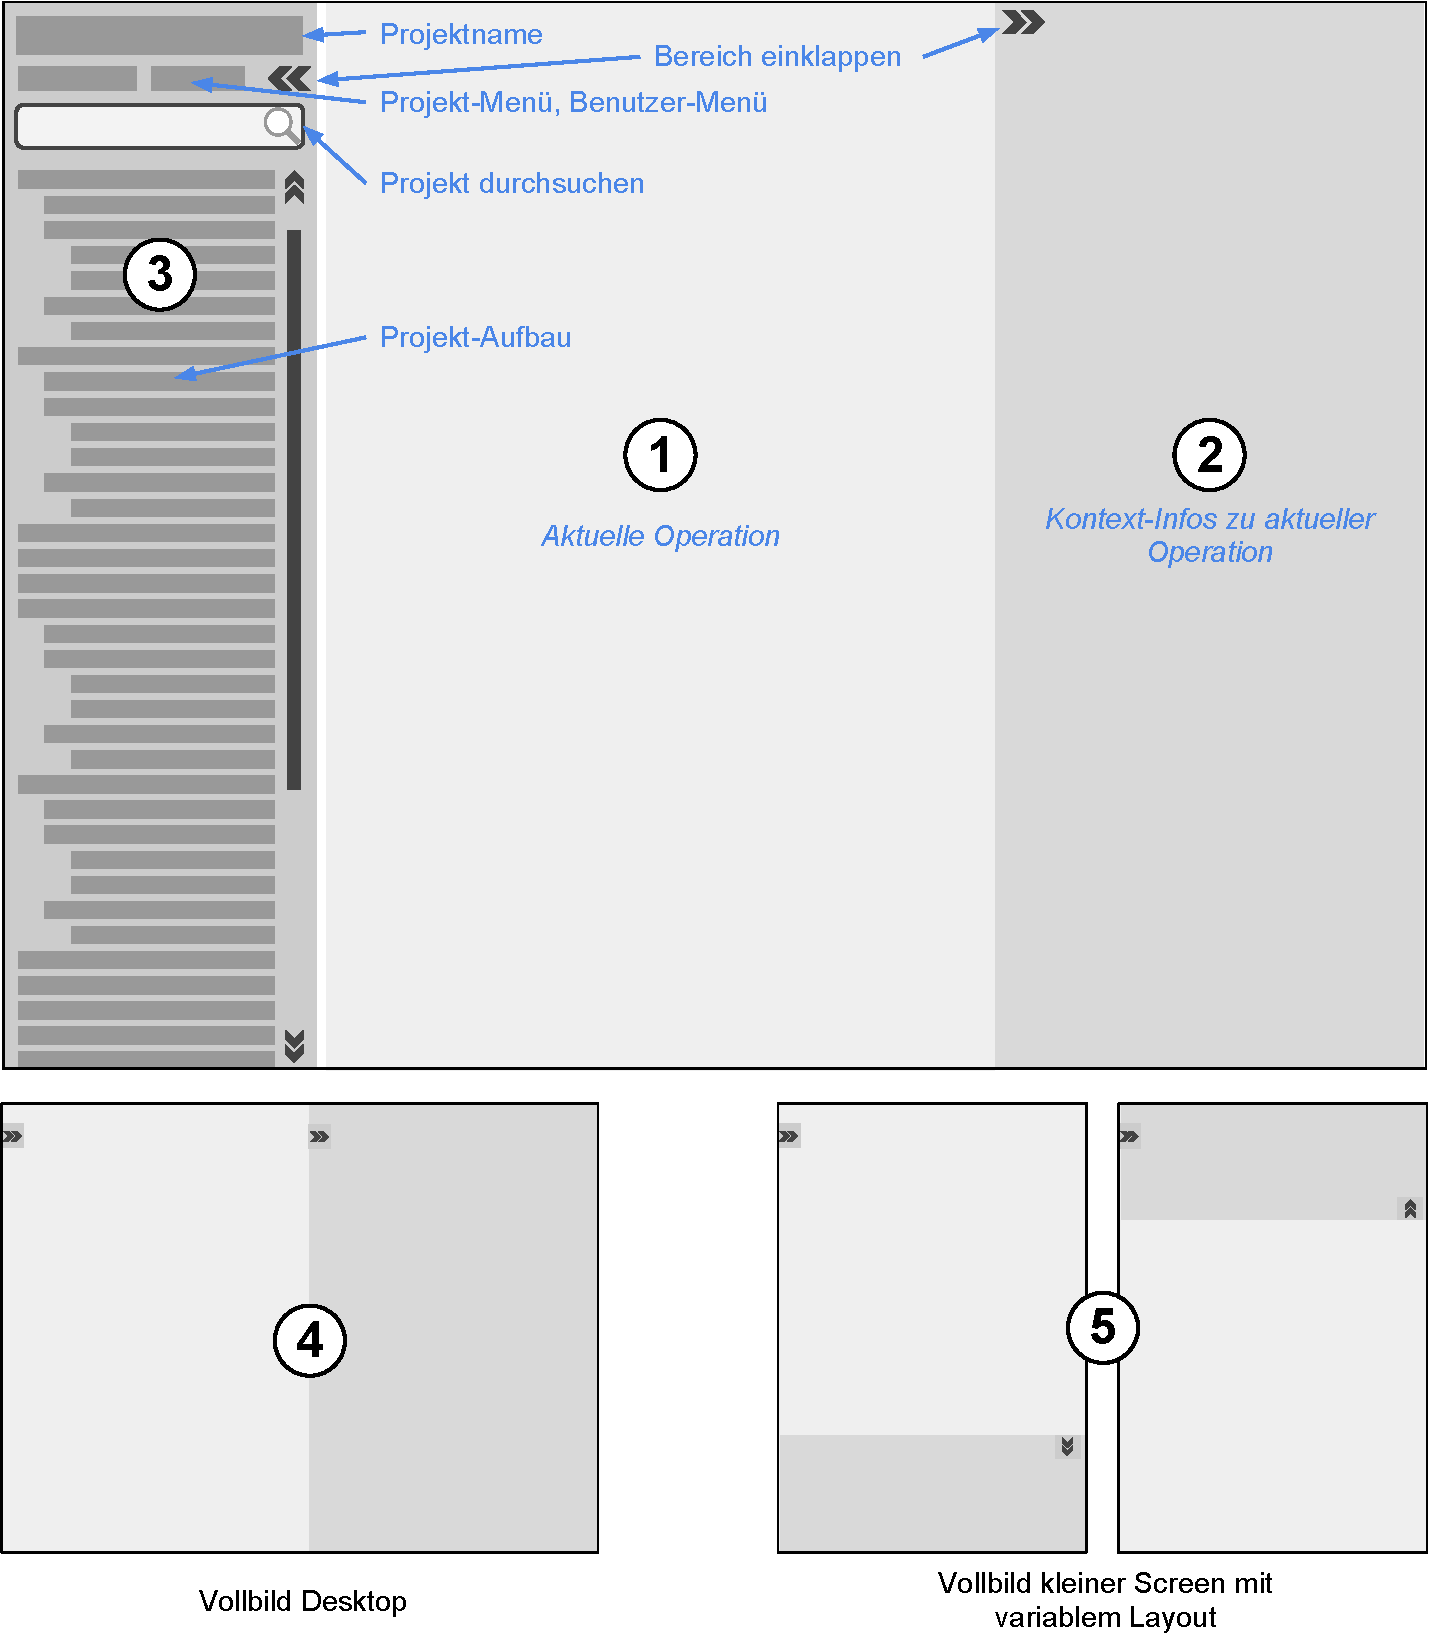
\includegraphics[width=0.95\textwidth]{media/GUIAufbau.pdf}
\captionof{wireframe}{Aufbau des browserbasierten GUIs}\label{chart:gui-aufbau}
\end{center}

Wireframe~\ref{chart:gui-aufbau} zeigt den Grundaufbau des GUIs. Zentraler Bereich ist die Darstellung der \emph{aktuellen Operation} \ball{1} mit den zugehörigen \emph{Kontext-Informationen} \ball{2}. Auf der linke Seite findet sich eine Spalte über die im Projekt navigiert werden kann \ball{3}. Um den Fokus auf die aktuelle Aufgaben zu verbessern sind die Kontext-Information und die Projektspalte ausblendbar \ball{4}. Das gesamte Layout passt sich flexibel an verschiedene Bildschirmgrößen und -formate an, zusätzlich kann die Position der Kontext-Information an die eigenen Vorlieben angepasst werden \ball{5}.

Die Projekt-Spalte \ball{3} bietet direkten Zugang zu allen Teilen des aktiven Projekts. Die Projektstruktur wird mit einem Navigationsbaum dargestellt, über den direkt zu den jeweiligen Abschnitten gesprungen werden kann. Über das Suchfeld lässen sich die Einträge im Baum filtern. In der Spalte befindet sich oben zur Orientierung der Names des aktiven Projekts. Über das ausklappbare Projektmenü gelangt man Teilen der Anwendung, die nicht direkt über die Texte erreichbar sind, z.B. Projektauswahl, Mitarbeiterverwaltung, Export. Über das ausklappbare Benutzermenü kann man sich ausloggen, sein Profil bearbeiten und persönliche Einstellungen anpassen.

\pagebreak

\subsubsection{Definieren des Produkts}\label{l:gui-definition}

\begin{center}
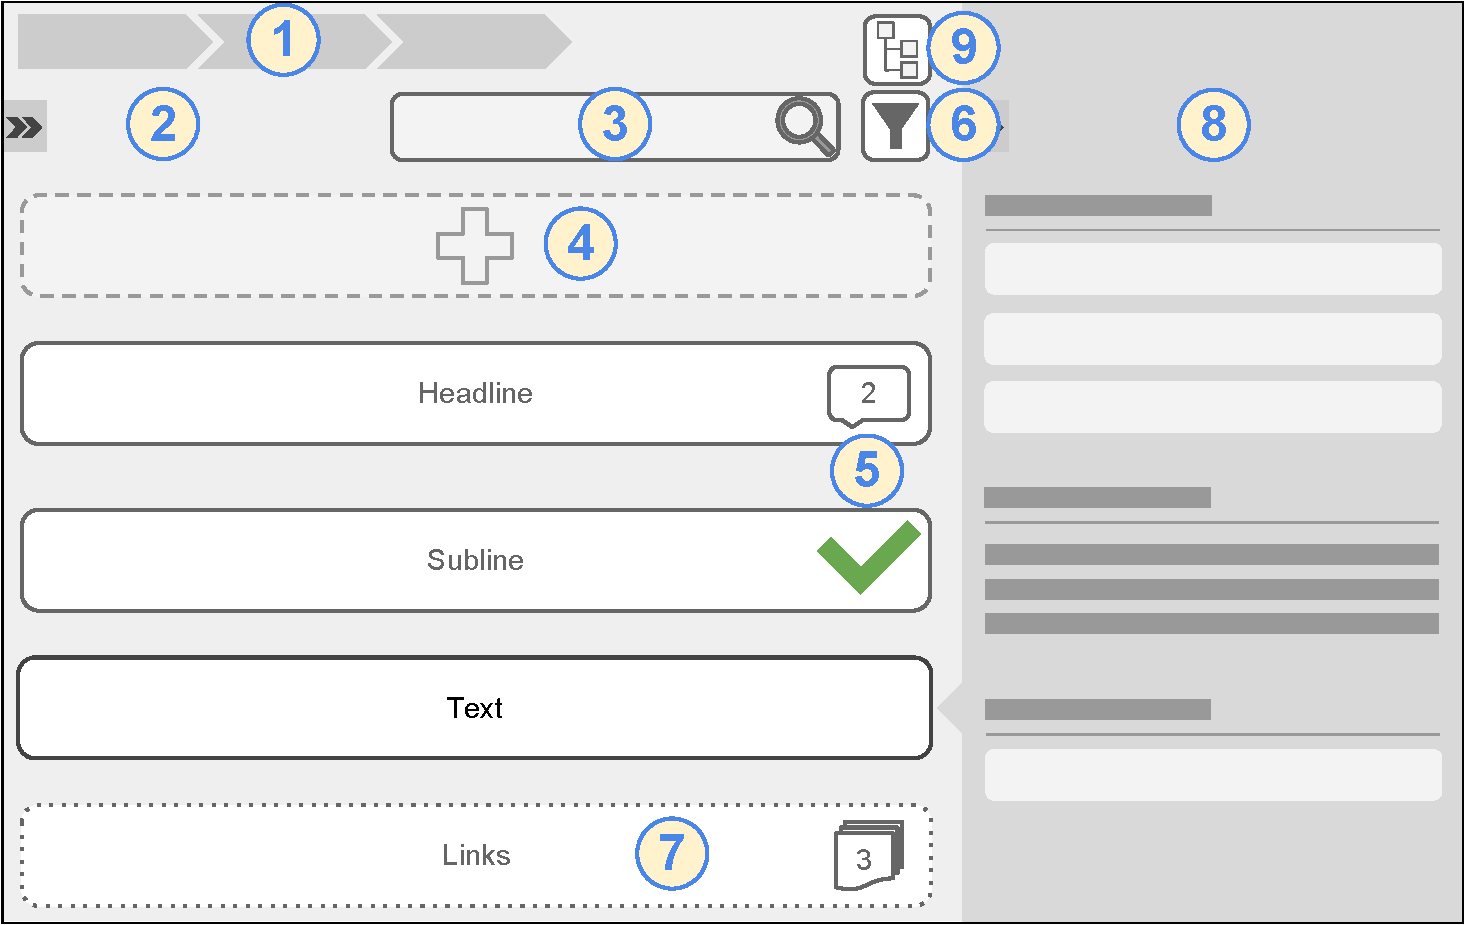
\includegraphics[width=0.95\textwidth]{media/GUIProduktstruktur.pdf}
\captionof{wireframe}{Bearbeiten der Produktstruktur}\label{chart:gui-produktstruktur}
\end{center}

Wireframe~\ref{chart:gui-produktstruktur} zeigt die Darstellung des GUIs zur Bearbeitung der Produktstruktur. Über die Breadcrumb-Navigation \ball{1}, die die aktuelle Position in der Projekthierarchie zeigt, ist eine Orientierung auch ohne das eingeklappte Projektmenü möglich. Über eine Schaltfläche lassen sich alle Container aber der aktuellen Hierarchiebene aufklappen, so ist können umfangreiche Änderungen an vielen Elementen gleichzeitig vorgenommen werden, ohne dass man sich durch die verschiedenen Ebenen \typoquotes{hangeln} muss. Im Inhaltsbereich \ball{2} werden die auf der aktuellen Ebene befindlichen Inhalts-Elemente, Textbausteine und Container, angezeigt. Die Darstellung erfolgt in eine kompakten Weise, die einen schnellen Überblick über die Inhalte bietet ohne viel Scrollen zu müssen. Die einzelnen Inhalts-Elemente können mit Drag\&Drop in ihrere Reihenfolge angepasst werden. Über das Suchfeld \ball{3} können die angezeigten Elemente gefiltert werden. Über eine Schaltfläche \ball{4} können neue Inhalts-Elemente erstellt werden. Zusatzinformationen wie der Typ, der Status, Kommentare oder ähnliche können auch verwendet werden, um die Inhalte auf der Seite zu filtern, z.B. um nur die Element anzuzeigen, für die noch die Inhalte fehlen \ball{5}. Durch Klick auf einen Container \ball{6} gelangt man eine Ebene tiefer, in diesen Conatiner hinein. Das Icon gibt die Anzahl der untergeordneten Element an. In der Spalte für die Kontext-Information \ball{7} werden Detailinformation zum aktuell ausgewählten Element dargestellt, die an die eingestellten Ansichts-Art angepasst sind. Hier findet sich auch die Bearbeitungshistorie und die Kommentare zu den Inhalts-Elementen.

Über eine Schaltfläche \ball{8} kann zwischen den vier Ansichten (Definieren~\ref{l:gui-definition}, Texten~\ref{l:gui-texten}, Übersetzen~\ref{l:gui-uebersetzen} und Kontrolle~\ref{l:gui-qs}), die die Inhaltselemente manipulieren, gewechselt werden.

\pagebreak

\subsubsection{Texte erstellen}\label{l:gui-texten}

\begin{center}
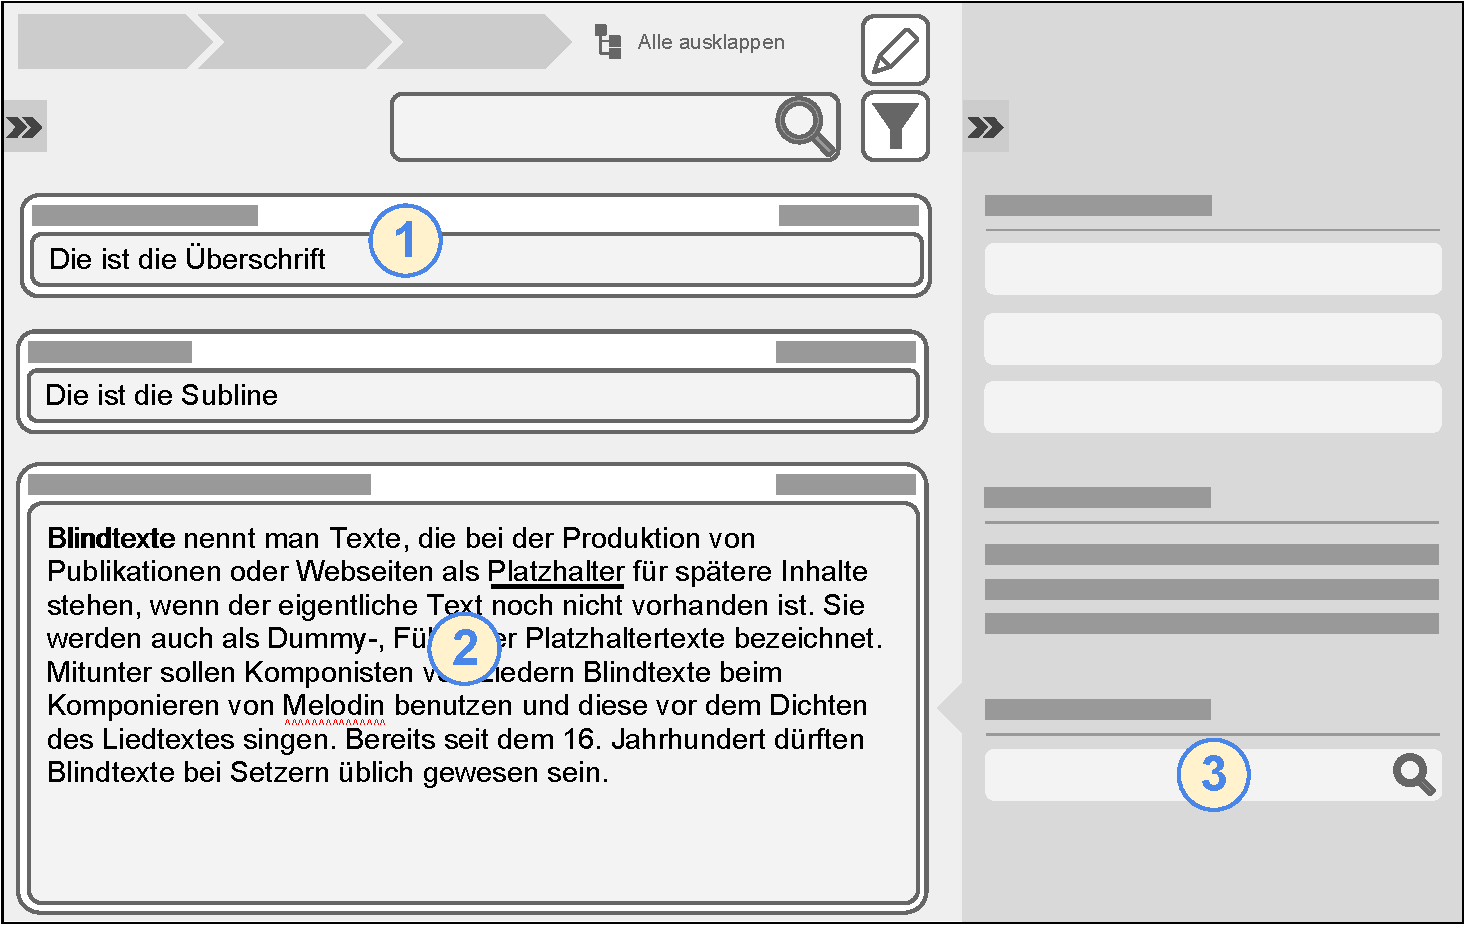
\includegraphics[width=0.95\textwidth]{media/GUITexteerstellen.pdf}
\captionof{wireframe}{Erstellen der Texte}\label{chart:gui-texten}
\end{center}

Wireframe~\ref{chart:gui-texten} zeigt die Darstellung des GUIs zur Bearbeitung der Texte des Produkts. Die Inhaltselemente in der aktuelle Hierarchie werden dabei mit Eingabefeldern für die Inhalte dargestellt \ball{1}. Links über dem Eingabefeld wird die Bezeichnung des Textbausteins angezeigt und rechts darüber Hinweise zu Längebeschränkungen (falls vorhanden) mit Zähler. Während der Eingabe können bereits Auszeichnungen vorgenommen werden, die Schaltflächen dazu, werden eingeblendet, sobald sich der Cursor im Feld befindet. Innerhalb der Kontext-Informationen \ball{3} besteht die Möglichkeit direkt eine Suche zu starten, die Suchergebnisse werden in einem Dialog-Fenster geöffnet. 

\pagebreak

\subsubsection{Texte übersetzen}\label{l:gui-uebersetzen}

\begin{center}
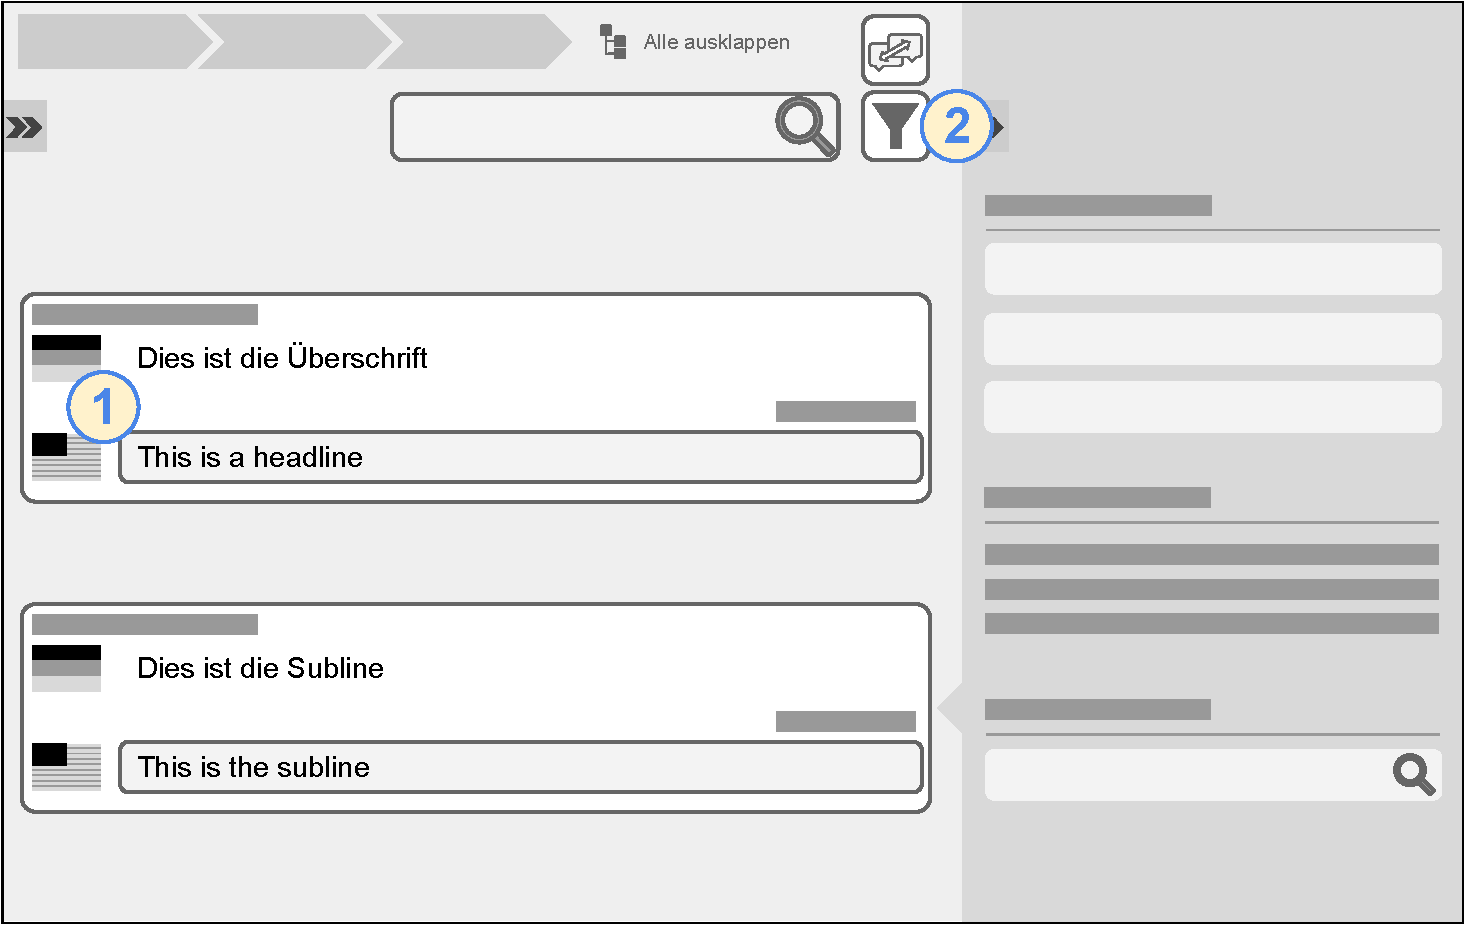
\includegraphics[width=0.95\textwidth]{media/GUITexteuebersetzen.pdf}
\captionof{wireframe}{Übersetzen der Texte}\label{chart:gui-uebersetzen}
\end{center}

Wireframe~\ref{chart:gui-uebersetzen} zeigt die Darstellung des GUIs zur Übersetzung der Texte des Produkts. Hierzu wird der Inhalt des Textbausteines in der Original-Sprache angezeigt und darunter ein Eingabefeld, in dem die Übersetzung eingetragen wird \ball{1}. Über einen Filter-Dialog \ball{2} kann konfiguriert werden, welche Sprachen angezeigt werden sollen.

\pagebreak

\subsubsection{Prüfen}\label{l:gui-qs}

\begin{center}
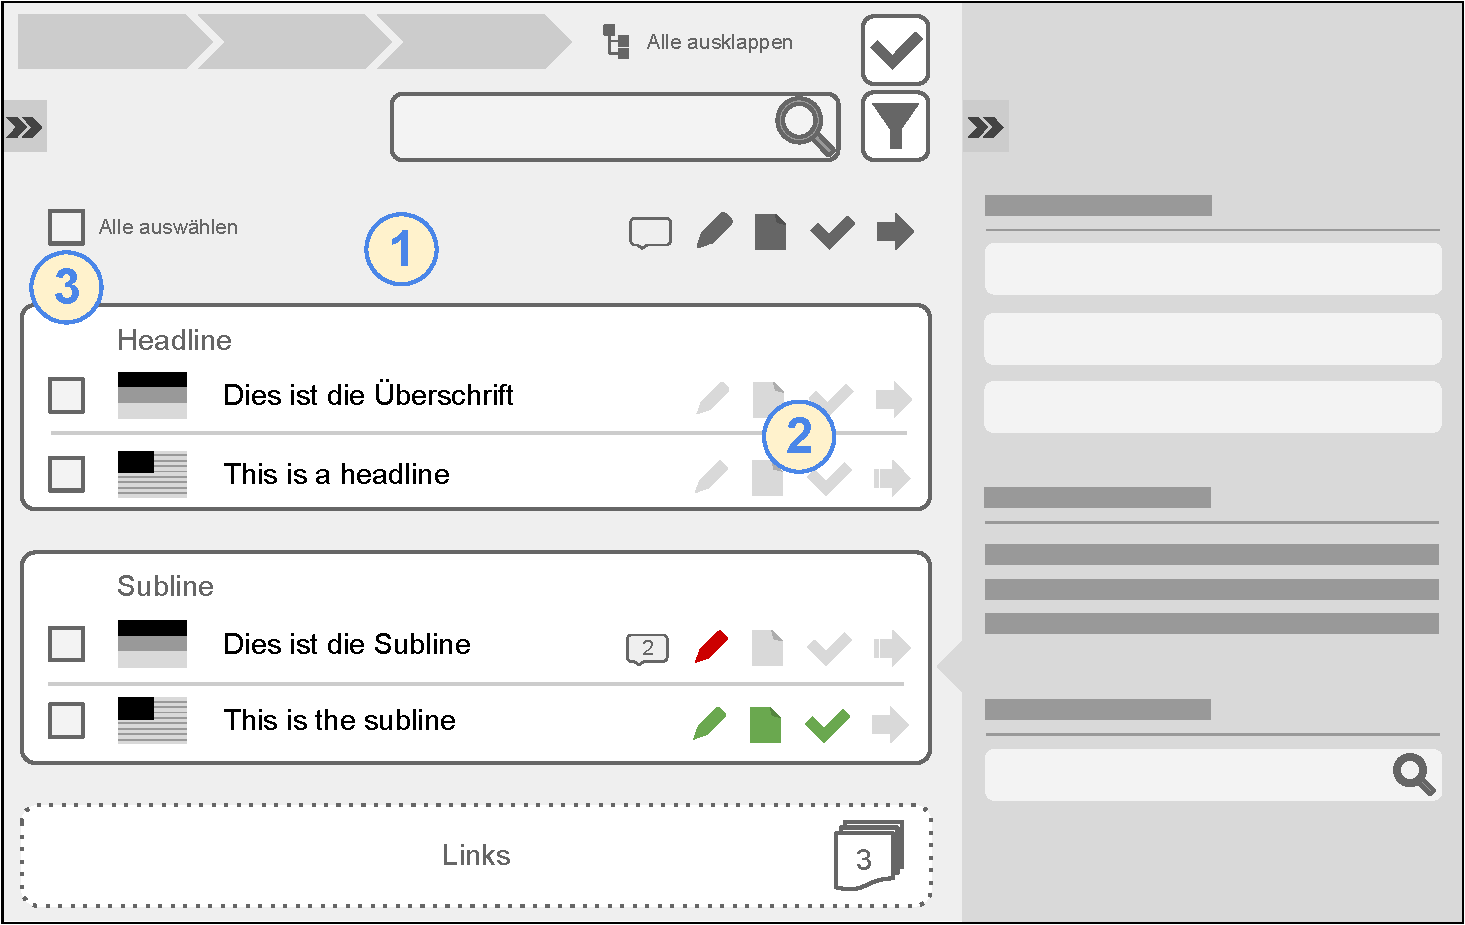
\includegraphics[width=0.95\textwidth]{media/GUIFreigabe.pdf}
\captionof{wireframe}{Überprüfen der Texte}\label{chart:gui-qs}
\end{center}

Wireframe~\ref{chart:gui-qs} zeigt die Darstellung des GUIs zur Kontrolle und Freigabe der Texte des Produkts. In dieser Ansicht werden die verschiedenen Stati der Textbausteine bearbeitet. Hierzu sind die Textbausteine mit ihren Übersetzungen dargestellt \ball{1}. Über die mit Icons markierten Schaltflächen \ball{2} lassen sich die einzelnen Stati direkt setzen. Von links nach rechts sind das: Korrigiert, Geprüft, Freigegeben und Veröffentlicht. Es wird jeweils zwischen \typoquotes{keine Angabe} (grau), \typoquotes{abgelehnt} (rot) und \typoquotes{in Ordnung} (grün) unterschieden. Hier wird auch die Anzahl der hinterlegten Kommentare angezeigt. Zum massenhaften bearbeiten von Stati können mehrere oder alle Elemente über die Checkboxen \ball{3} ausgewählt werden. Über die Status-Icons in der Kopfzeile kann dann der Status für alle ausgewählten Elemente gleichzeitig gesetzt werden.

\pagebreak

\subsubsection{Kontext-Informationen}\label{l:gui-kontext}

\begin{center}
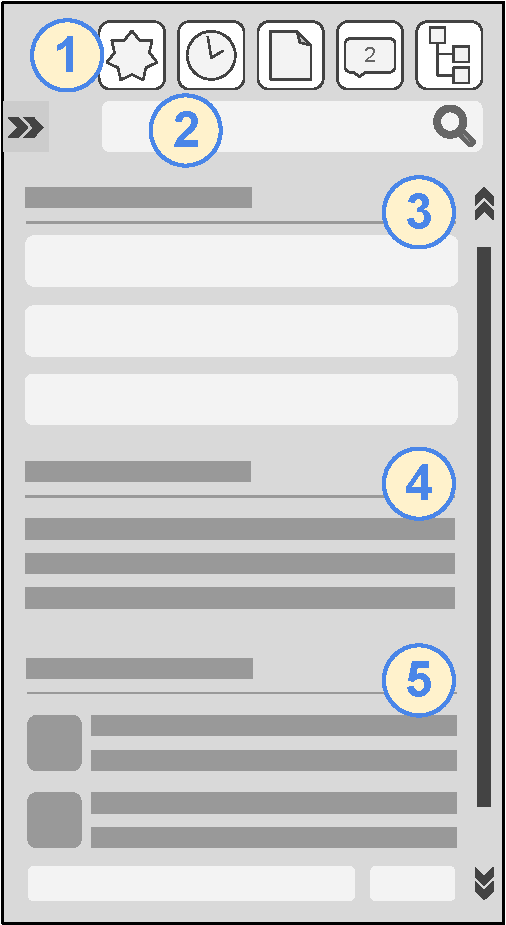
\includegraphics[width=0.35\textwidth]{media/GUIKontext-Informationen.pdf}
\captionof{wireframe}{Kontext-Informationen}\label{chart:gui-kontext}
\end{center}

Wireframe~\ref{chart:gui-kontext} zeigt die Darstellung des GUIs zur Anzeige und Bearbeitung der Kontext-Informationen. Der Inhalt der Ansicht ist an die jeweilige Operation angepasst. Im oberen Bereich kann zwischen verschiedenen Kontextinformationen zu dem jeweiligen Inhalt umgeschaltet werden \ball{1} (v.l.n.r): 

\begin{enumerate}\itemsep -5pt
\item Neues: Listet die neuesten Informationen aus den vier Bereichen und den aktuellen Status.
\item Änderungshistorie: Zeigt die vergangenen Änderungen an, mit der Möglichkeit, diese zu kommentieren und zurückzunehmen.
\item Material: Zeigt hinterlegte Materialien an. Dabei handelt es sich um Dateien und Freitext-Notizen.
\item Kommentare: Zeigt die Kommentare an.
\item Struktur: Zeigt Informationen zur Struktur innerhalb des Produkts, wie z.B. die Attribute, an.
\end{enumerate}

Über das Suchfeld \ball{2} lässt sich die aktuellen Ansicht filtern. In den Kontextinformation findet sich direkter Zugang zu Informationen und Operationen bezogen auf den aktuellen Inhalt. Die Inhalte lassen sich über Formulare \ball{3} direkt bearbeiten, Notizen und Dateien werden angezeigt \ball{4} und der Diksussion mithilfe der Kommentarfunktion ist möglich \ball{5}.

\pagebreak

\secbar

Die in diesem Abschnitt gezeigten Wireframes sind die Vorlage für eine mögliche Implementierung. Bei der Umsetzung des Protypen wurde versucht, dieser Vorlage weitestgehend zu folgen, wie in Abschnitt \ref{l:implementierung-gui} · S.\pageref{l:implementierung-gui} beschrieben wird. Im nächsten Abschnitt wird jedoch zuerst auf die Verbindung des Anwendungsservers mit einem GUI eingegangen.

\pagebreak

\subsection{Anbindung der GUI an den Anwendungsserver}\label{l:anbindung-gui}

Die in Abbildung~\ref{chart:komponenten} · S.\pageref{chart:komponenten} \emph{gelb} eingezeichneten Komponenten zeigen den Aufbau eines browserbasierten GUIs. Mittlerweile ist es üblich, klassische Paradigmen aus der Softwarentwicklung auch in browserbasierten Anwendung zu verwenden. Dementsprechend wird die GUI in Form einer MVC-Anwendung implementiert. Die Kommunikation mit dem Anwendungsserver wird in einer eigenen Komponente, dem \emph{API-Adapter}, gekapselt, die über die REST-Schnitt"-stelle JSON-Daten mit dem Anwendungsserver austauscht. Die Repräsentation der Domänendaten erfolgt dabei mithilfe von entsprechenden \emph{Models}, die durch die \emph{Controller} mit den \emph{Views} verbunden werden. Die Models sind nicht zwangsläufig mit den Models auf der Serverseite identisch sondern können Aggregationen sein, oder nur Teile der Daten abbilden, sie orientieren sich an der öffentlichen API des Anwendungsserver, die nicht zwingenderweise die interenen Models 1:1 nach außen weiterreicht. Views sind einzelne Bestandteile einer Ansicht. So lassen sich individuelle Bereiche der Darstellung leicht aktualisieren, ohne die ganze Seite neu laden zu müssen -- in \cite[S.1--5 und S.65--72]{maccaw2011javascript} ist dieses Prinzip ausführlich erläutert.

Ein Problem beim Datenaustausch mithilfe von JSON-Objekten ist, dass diese üblicherweise nur reine Daten enthält, da schlichterweise Objekte serialisiert werden. Beim Serialisieren werden dann nur die Eigenschaften einer Objekt-Instanz beibehalten, Informationen wie die Klasse oder Relationen zu anderen Objekten werden verworfen. Werden APIs nach diesem Schema verwendet, müssen die Entwickler wissen, hinter welchem Endpunkt sie welche Arten von Daten erwarten. Diese Information wird als Quellcode hart kodiert. Um zukünftigen Änderungen an der Schnittstelle ohne Änderungen auf Clientseite begegnen zu können sollten die Antworten der Schnittstelle mit Meta-Informationen versehen sein, die es dem Client ermöglichen, ohne hart kodierte Zuordnung zwischen Endpunkt und Domänenobjekt auszukommen. 

\begin{samepage}
\trademark{JSON-LD}\footnote{\url{http://json-ld.org/}} hat sich dabei als Lösung bewährt. Hierbei werden JSON-Objekt mit Me"-ta-In"-for"-mat"-ion"-en versehen, die beschreiben, um \emph{was} für ein Objekt es sich bei der Antwort handelt (\texttt{@context}) und um \emph{welches} (\texttt{@id}):

\begin{verbatim}
{ "@context": "http://json-ld.org/contexts/person.jsonld",
  "@id": "http://dbpedia.org/resource/John_Lennon",
  "name": "John Lennon",
  "born": "1940-10-09",
  "spouse": "http://dbpedia.org/resource/Cynthia_Lennon" }
\end{verbatim}
\end{samepage}

In dieser Art kann ein JSON-Objekt auch mit Informationen über zugehörige \emph{andere} Objekte versehen werden. Im Beispiel verweist \texttt{spouse} auf die URL unter der das JSON-Objekt der Ehefrau abgerufen werden kann. Auf diese Weise lassen sich die vollständige Datenstruktur einer Anwendung als Graph darstellen. Hierzu werden alle Objekte mit Relationen annotiert und der Client kann entscheiden, welchen Relationen er folgt und welchen nicht. Die die Relations-Informationen auch die URLs zu den Endpunkten enthalten, müssen in der Implementierung keine Endpunkte mehr hart codiert werden, es ist lediglich nötig, einen Einstiegs-Punkt zu kennen von dem aus man mit sich durch den Graphen \typoquotes{hangeln} kann, indem man Objekt-Relationen folgt, deren Kontexte die Anwendung erkennt.\footnote{\url{http://coderbyheart.de/blog/relationen-in-linked-data}}

\pagebreak

\subsection{Implementierung des GUI}\label{l:implementierung-gui}

Im Prototyp wurden das GUI als reine JavaScript-Anwendung umgesetzt. Als Framework für den Aufbau der Anwendung wurde \trademark{Backbone.js}\footnote{\url{http://backbonejs.org/}} eingesetzt. 

\subsubsection{Komponenten}

\trademark{Backbone.js} stellt Basisklassen für Models, Views und Collections (Listen von Models) zur Verfügung, die mit Hilfe eines zentralen Routers zu einer Anwendung verbunden werden können, die mit einer RESTful-API kommunziert. Der Router übernimmt dabei die Aufgabe, abhängig von der URL im Browser zu steuern, welche View gerade eingezeigt wird. 

Um die einzelnen Bestandteile der Anwendung möglichst modular zu halten und Ladezeiten so kurz wie möglich zu halten, kommt \trademark{require.js}\footnote{\url{http://requirejs.org/}} zum Einsatz, mit dessen Hilfe es möglich ist, nur die für den aktuellen Code-Pfad nötigen Abhängigkeiten zu laden. Neben dem Nachladen von Ja\-va\-Scr\-ipt-Code ist es damit auch möglich HTML-Dateien nachzuladen, dies wird in der Implementierung dazu verwendet, den HTML-Code zur Darstellung der Anwendung ebenfalls modular und nur bei Bedarf nachzuladen. Dies ermöglich zudem eine saubere Trennung zwischen der Darstellungslogik, die in JavaScript implementiert ist und dem zugehörigen HTML-Quellcode. \trademark{Underscore.js}\footnote{\url{http://underscore.org/}}, auf dem \trademark{Backbone.js} aufbaut, liefert hierzu einfache Templating-Funktionen.

Zur Realisierung der GUI-Funktionalität wurde \trademark{Twitter Bootstrap}\footnote{\url{http://twitter.github.com/bootstrap/}} eingesetzt, ein HTML5-Framework, das für viele GUI-Elemente bereits vorgefertigte Darstellungen bietet. Einige Elemente werden mit Hilfe von JavaScript mit erweiterter Funktionalität versehen, in \trademark{Twitter Bootstrap} kommt dabei \trademark{JQuery}\footnote{\url{http://jquery.com/}} zum Einsatz. \trademark{Twitter Bootstrap} ermöglich von sich aus das GUI \emph{responsive} zu implementieren, d.h. dass keine festen Maßangaben verwendet werden. So ist eine saubere Darstellung auf vielen unterschiedlichen Endgeräte sichergestellt. Mit Hilfe von \emph{CSS media queries} können einfach Anpassung für bestimmte Bildschirmgrößen implementiert werden.

Alle genannten Komponenten sind umfangreich getestet und funktionieren in allen aktuellen Browsern und sind auch abwärtskompatibel zu älteren Browsern.

\setlength\fboxsep{2pt}
\setlength\fboxrule{0.5pt}

\begin{center}
\fbox{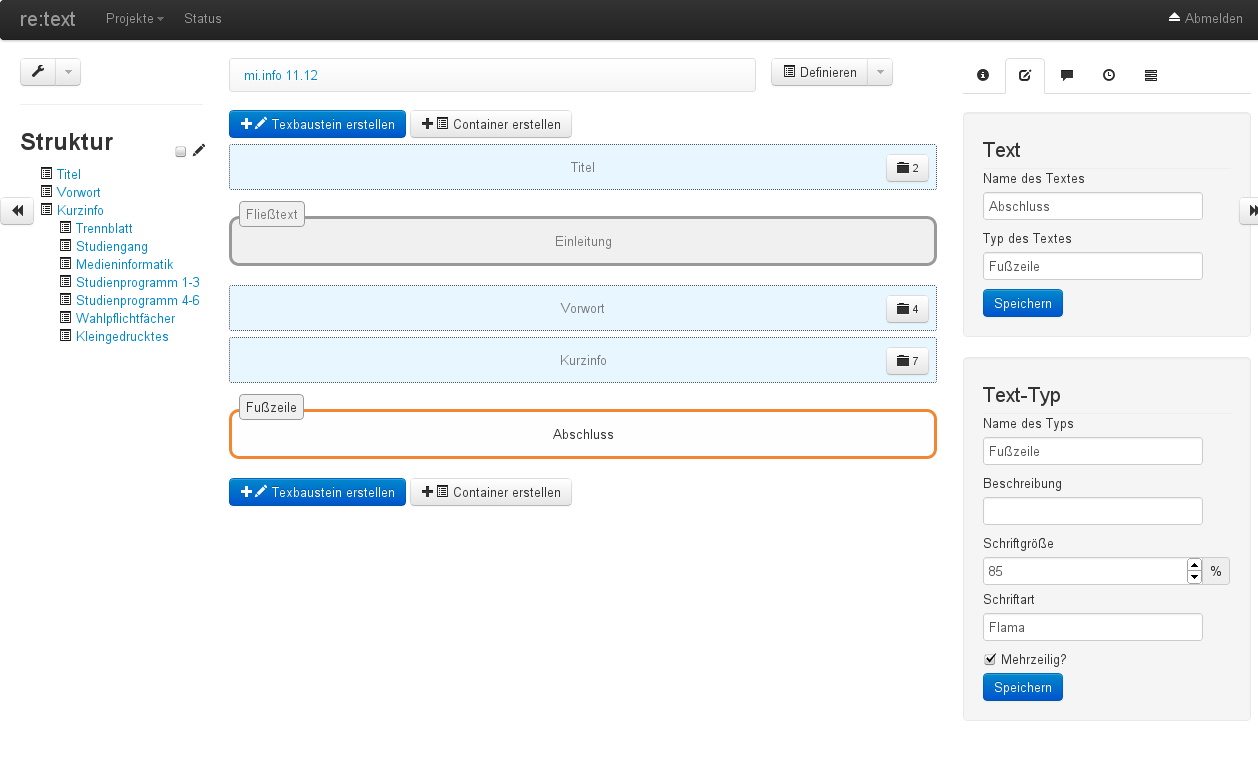
\includegraphics[width=\textwidth]{media/screenshots/app.png}}
\captionof{screenshot}{Browserbasiertes GUI des Prototyps}\label{chart:gui-prototyp}
\end{center}

Screenshot~\ref{chart:gui-prototyp} zeigt den Aufbau des GUI des Prototyps beispielhaft in der Ansicht zur Definition des Produkts (vgl. Abschnitt \ref{l:gui-definition} / \pageref{l:gui-definition}). Die Anordnung der Elemente des Entwurfs wurde weitgehend beibehalten. Unterschiede resultieren aus im Prototyp nicht implementierte Funktionen, die nicht mit Platzhalter-Elementen dargestellt werden, sondern entfallen. Weitere Screenshots finden sich in Anhang~\ref{l:screenshots} · S.\pageref{l:screenshots}.

\subsubsection{Klassendiagramm}

\begin{center}
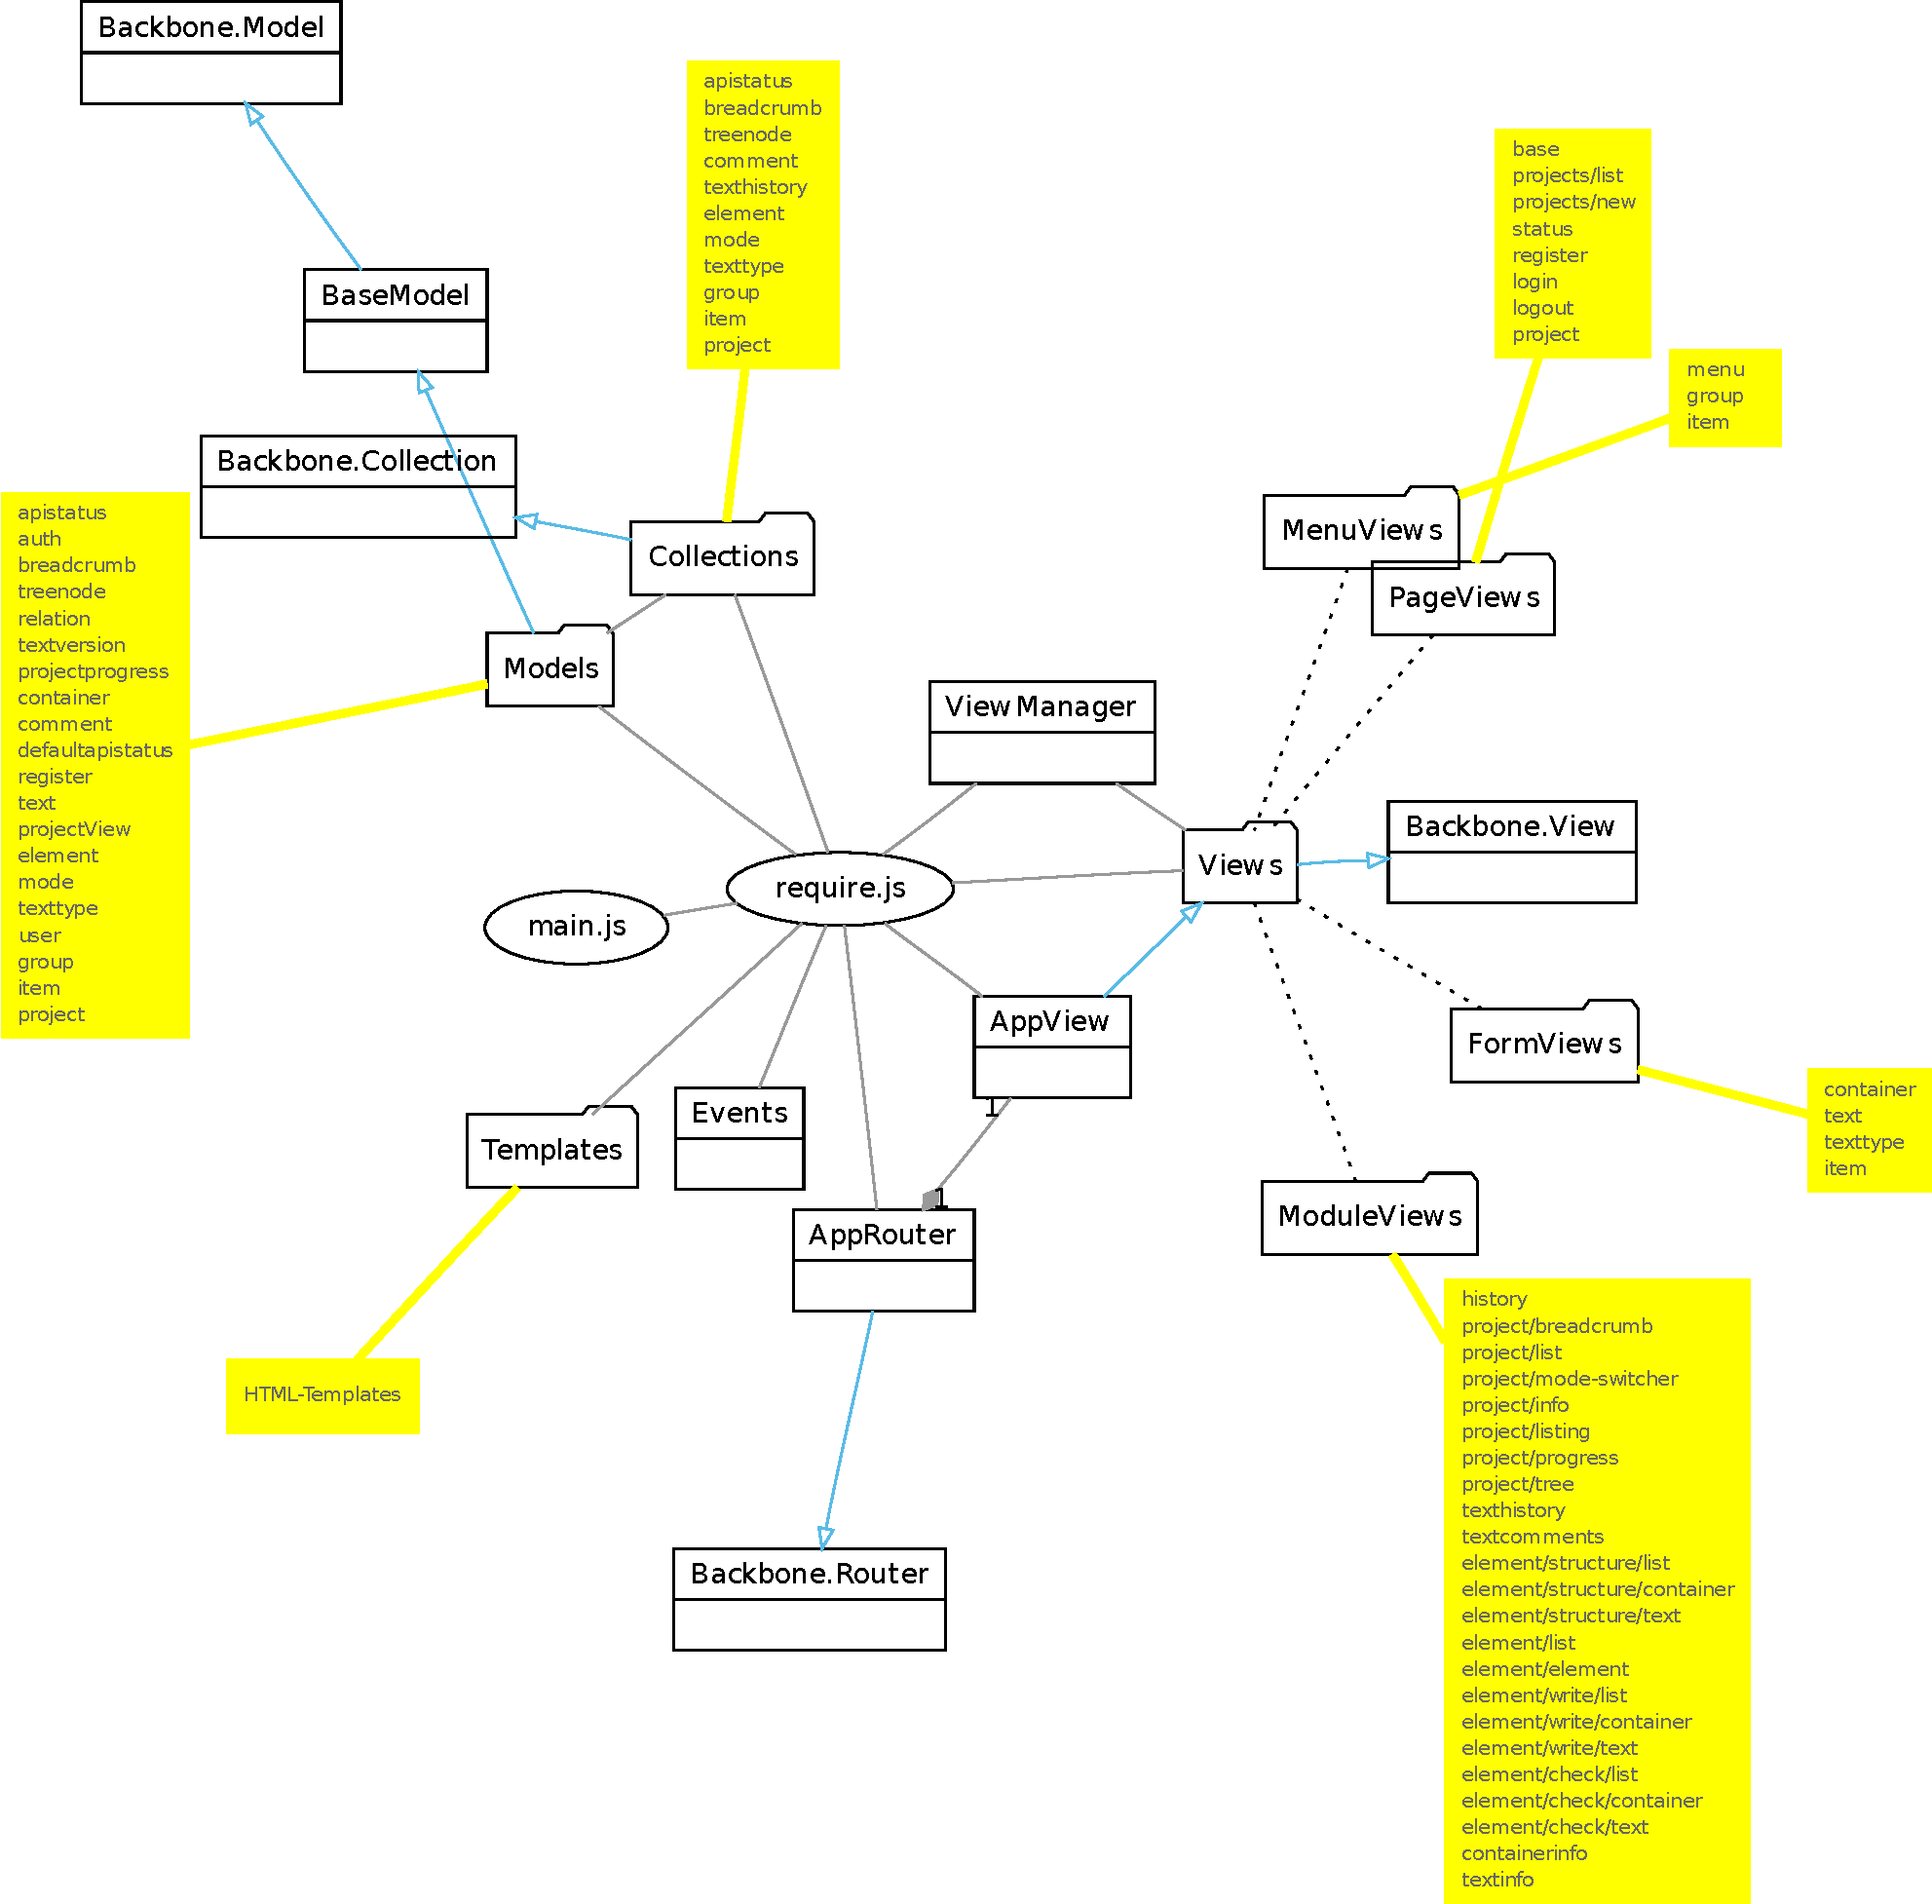
\includegraphics[width=\textwidth]{media/prototyp-gui-klassendiagramm.pdf}
\captionof{figure}{GUI-Klassendiagramm des Prototyps}\label{chart:prototyp-gui-klassendiagramm}
\end{center}

Abbildung \ref{chart:prototyp-gui-klassendiagramm} zeigt das Klassendiagramm der browserbasierten Anwendung. Zentraler Einstiegspunkt ist die JavaScript-Datein \texttt{main.js}, die die Anwendung initialisiert. Dazu lädt sie mit Hilfe von \texttt{require.js} die notwendigen Komponenten. Dabei handelt es sich zum einem um die \texttt{AppView}, die grundlegende Zustände der Anwendung verwaltet und den \texttt{AppRouter}, der je nach aktueller Route die jeweilige \texttt{PageView} initialisiert und anzeigt. Die \texttt{PageViews} erzeigen danach wiederum eiogenständig die von ihnen benötigten Ansichten (\texttt{ModuleViews}, \texttt{MenuViews} und \texttt{FormViews}) und Laden die dafür benötigten Daten mithilfe der \texttt{Models} und \texttt{Collections} -- in \trademark{Backbone.js} sind \emph{Views} eigentlich Controller, eine Trennung zwischen Darstellungslogik und Businesslogik ist nicht vorgesehen. Den HTML-Quellcode zur Darstellung laden die Views ebenfalls selbständig aus den \texttt{Templates} nach. Abhängigkeiten wie JavaScript-Objekte und Templates werden dabei zentral von \trademark{require.js} bereitgestellt, dass damit die Aufgabe eines DI-Containers übernimmt und praktisch auch so verwendet werden kann.

Die Kommunikation mit der API wird durch die \trademark{Backbone.js}-Klassen \texttt{Backbone.Model} und \texttt{Backbone.Collection} abstrahiert, die RESTful-APIs ansprechen können, die dem CRUD-Paradigma entsprechen. Siehe dazu die Beschreibung der API-Implementierung in Abschnitt \ref{l:api-implementierung} · S.\pageref{l:api-implementierung}.

\secbar

Das browserbasierte GUI ist zwar eine eigenständige Anwendung, ohne einen Anwendungsserver lässt sich hiermit jedoch nicht arbeiten, da die GUI lediglich zum Darstellen und modifizieren von Daten verwendet wird, die Persistenz und vor allem die Sicherung von Datenzugriffen, Berechtigungen, sowie viele weitere Funktionen werden im Anwendungsserver implementiert, der im nächsten Abschnitt beschrieben wird.

\pagebreak

\subsection{Entwurf des Anwendungsservers}\label{l:entwurf-server}

In diesem Abschnitt werden die in Abbildung~\ref{chart:komponenten} · S.\pageref{chart:komponenten} grau eingefärbten Komponenten des Anwendungsservers beschrieben.

\subsubsection{API, Cronjobs, CLI, …}

In der API-Komponenten, die als REST-API implementiert ist, sind über eine Rou"-ting-Ta"-bel"-le alle Controller registriert. Da das System mit einer vollständigen Abdeckung aller Operation durch API-Endpunkte implementiert ist, wird diese auch lokalen ausgeführten Scripten wie z.B. Cronjobs oder CLIs verwendet. Dies ermöglicht eine saubere Trennung, auch für administrative Aufgaben, und verhindert, dass Sonderfälle oder Workarounds für bestimmte Aufgaben kultiviert werden.

\subsubsection{Dependency-Injection-Container}

Der einzelnen Komponenten des Anwendungsservers sind nach dem Prinzip der losen Kopplung verbunden (vgl.~\cite[S.62]{hn-web20}). Hierzu werden die einzelnen Komponenten als Services in einem Dependency-Injection-Container (DI-Container) registriert und von diesem instanziiert. Alle Komponenten können auf den DI-Container zugreifen und dort andere Komponenten anfordern. Der DI-Container übernimmt, wie der Name schon sagt, auch die Aufgabe Abhängigkeiten der einzelnen Komponenten bereitzustellen. Ein so aufgebautes System, bei dem konkrete Instanzen nicht mehr an der Stelle erzeugt werden, an der sie verwendet werden, sondern von außen \typoquotes{hereingereicht} werden, ist leicht zu modifizieren und vor allem leicht zu testen, da sich Abhängigkeiten für Tests leicht durch Mock-Objekte austauschen lassen (vgl.~\cite[Kap.2]{freeman2009growing}).

\subsubsection{Controller}

Zentrale Komponente bilden die Controller. Hier ist die Business-Logik der Anwendung implementiert. Die einzelnen Operationen sind in verschiedenen Controllern implementiert, so ist das System leicht erweiter- und wartbar. Die Controller werden von der API-Komponente entsprechende den Routen instanziiert, für die sie registriert sind. Controller haben über den DI-Container Zugriff auf alle Teile des Systems und erzeugen die Antwort auf eine Anfrage, die mit der API-Komponenten an den Client zurückgeschickt wird.

\subsubsection{Models}

Zu den Kern-Komponenten gehören auch die Models. Diese können ohne den DI-Container direkt von den jeweiligen Komponenten instanziiert werden, da sie reine Datenobjekt sind und weder Logik enthalten, noch Abhängigkeiten besitzen. Siehe hierzu auch das Domänenmodell auf S.\pageref{l:domänenmodell}.

\subsubsection{Persistenz, ORM}

Mit dieser Komponente werden die innerhalb der Anwendung erzeugten Daten persistiert. Mithilfe eines Object-Relational-Mappers (ORM) werden die Domänendaten, die durch die Models ausgedrückt werden, in relationale Daten umgewandelt, sofern zur Datenspeicherung ein relationales Datenbanksystem (RDBMS) verwendet wird. Wird hier eine nicht-relationale Datenbank (Dokumentendatenbank, Key-Value-Store) verwendet, kann der ORM entfallen bzw. wird durch ein entsprechende Komponente ersetzt.

\subsubsection{Import/Export \& Benachrichtigung}

\begin{center}
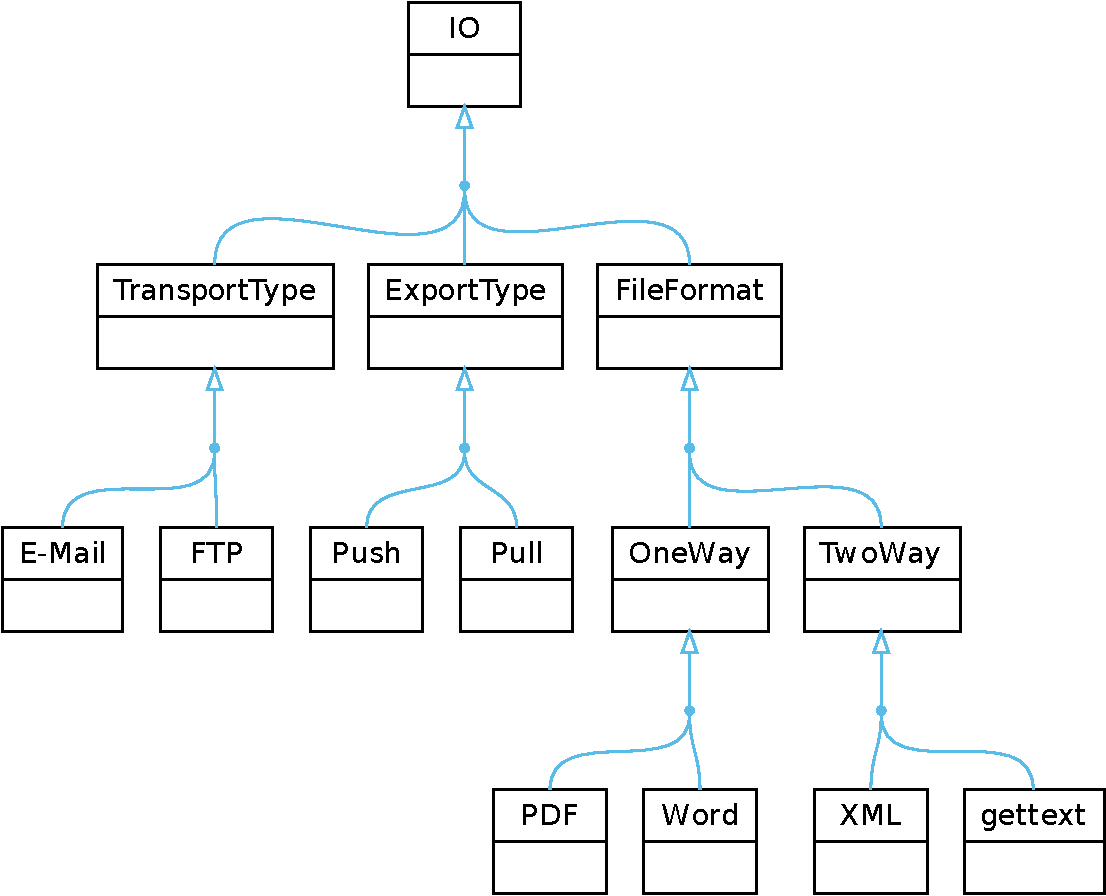
\includegraphics[width=0.75\textwidth]{media/io.pdf}
\captionof{figure}{IO-Komponente}\label{chart:io}
\end{center}

Diese Komponente ist für den Import von Daten aus verschiedenen Formaten in das interne Repräsentationsmodell und den umgekehrten Export zuständig. Die Komponente ist unterteilt in drei Bereiche, die nach dem Transport-Weg (z.B. E-Mail oder FTP), der Art des Ex- oder Importes (synchron, asynchron bzw. Push oder Pull) und nach dem Dateiformat unterscheiden (vgl.~Abb.~\ref{chart:io}).  Hierbei gibt es synchrone Exporte, z.B. den Download eines Exports über die Schnittstelle und asynchrone Exporte, z.B. den Upload auf einen FTP-Server. Benachrichtigungen sind ebenfalls in dieser Komponente implementiert, eine Benachrichtigung ist z.B. ein asynchroner Export via E-Mail, wobei keine Daten exportiert werden, sondern z.B. nur die Informationen zu einem Ereignis.

\subsubsection{Jobs}

Zeitaufwändige und wiederkehrende Operation wie z.B. der Datenimport oder das Versenden von Benachrichtigungen werden mithilfe von Jobs verarbeitet. Die Informationen zu einem Job werden in die Message-Queue eines Job-Server eingestellt und von dort registrierten Job-Runnern verarbeitet.

\subsubsection{Workflow}

In der Workflow-Komponente sind die Funktionen zur Definition und Ablaufsteuerung von komplexeren Workflows implementiert.

\subsubsection{Service-Adapter}

Über Service-Adapter werden externe Dienste oder andere Softwarekomponenten angebunden, die bestimmte Funktionen für die Anwendung zur Verfügung stellen, z.B. Wörterbücher, Datei-Konverter usw.

\secbar

Die in diesem Abschnitt vorgestellten Komponenten bilden gemeinsam ein umfangreiches, komplexes System, mit dem sich alle Anforderungen abbilden lassen. Der im nächsten Abschnitt beschriebene Prototyp verwendet aufgrund seines sehr überschaubaren Funktionsumfangs nur einen Teil der genannten Komponenten. Es wird jedoch darauf geachtet, die Implementierung möglichst nahe an dieser Vorlage zu realisieren.

\pagebreak

\subsection{Implementierung des Anwendungsservers}\label{l:implementierung-server}

Für den Prototyp wurde das PHP-Framework \trademark{Symfony2}\footnote{\url{http://symfony.com/}} eingesetzt, das von sich aus bereits viele Anforderungen des vorangegangenen Abschnitts erfüllt. 

\subsubsection{Kern-System}

Da im Kern jeder Web-Anwendung HTTP-Anfragen beantwortet werden, überträgt \trademark{Symfony2} dieses Paradigma auf die Art und Weise, wie im Framework Anfragen verarbeitet werden: mit Hilfe einer Routen-Konfiguration werden Controller für bestimmt Pfade in der Anfrage-URL registriert und dann bei Bedarf vom Framework automatisch instanziert und aufgerufen. 

Das folgende Listing zeigt die am Beispiel des \texttt{LoginControllers}, in dem die Methode \texttt{loginAction} aufgerufen wird, wenn der Pfad \texttt{\/login} lautet und die HTTP-Methode der Anfrage \texttt{POST} ist.

\begin{samepage}
\begin{verbatim}
class LoginController extends Base {
    /**
     * @Route("/login", requirements={"_method":"POST"})
     */
    public function loginAction() { … }
}
\end{verbatim}
\end{samepage}

Die Controller schreiben ihre Antwort in ein Objekt, das vom Framework als Antwort gesendet wird. Oberstes Prinzip bei der Entwicklung des Frameworks war die Modularisierung und die Wiederverwendbarkeit, so sind alle Komponenten ohne harte Abhängikeiten mithilfe eines DI-Containers verbunden. Dadurch sind \trademark{Symfony2}-Anwendungen besonders leicht zu warten und auch zu testen, entsprechende Unit-Testing-Komponenten werden bereits mitgeliefert.

\subsubsection{API}\label{l:api-implementierung}

Die API des Anwendungsservers wurde als RESTful-API implementiert und deckt alle Funktionen des Anwendungsservers ab. Sie folgt dem CRUD-Paradigma und unterstützt dementsprechen die jeweiligen Methoden: \texttt{POST} zum Erzeugen von (CREATE), \texttt{GET} zum Lesen von Daten (READ), \texttt{PUT} zum Aktualisieren bestehender Daten (UPDATE) und \texttt{DELETE} zum Löschen von Daten. Datenobjekte werden als JSON-Objekte übertragen, bei \texttt{GET}-Anfragen sind URL-Parameter zulässig. Eine Aufstellung aller implementierten API-Endpunkte findet sich in Anhang \ref{l:api-endpoints} · S.\pageref{l:api-endpoints}.

Die ausgelieferten JSON-Objekte enthalten Zusatzinformationen zum Kontext und zu Relationen, wie in Abschnitt \ref{l:anbindung-gui} · S.\pageref{l:anbindung-gui} beschrieben. 

\begin{samepage}
\begin{verbatim}
{   "@context":"http://jsonld.retext.it/Container",
    "@id":"/api/container/4fdf26e7820b905118000001",
    "@relations":[
        {
            "@context":"http://coderbyheart.de/jsonld/Relation",
            "relatedcontext":"http://jsonld.retext.it/Project",
            "href":"/api/project/4fdf26e7820b905118000000",
            "list":false
        },
        {
            "@context":"http://coderbyheart.de/jsonld/Relation",
            "relatedcontext":"http://jsonld.retext.it/Element",
            "role":"http://jsonld.retext.it/ontology/child",
            "href":"/api/element?parent=4fdf26e7820b905118000001",
            "list":true
        },
        …
    ],
    "id": "4fdf26e7820b905118000001",
    "name": "Abschnitt 1",
    … }
\end{verbatim}

Dieses Listing zeigt als Beispiel das JSON-Objekt eines Containers. In der \texttt{@relations}-Liste ist der Verweis auf das Eltern-Element enthalten, aber auch auf die Liste mit untergeordneten Elementen dieses Containers. Im Client werden die Relationen je nach Bedarf durchsucht und die passende ausgewählt, sofern weitere Daten benötigt werden. Die jeweilige URL ist in \texttt{href} enthalten, so dass sich im Quellcode des Clients nur wenige hart-kodierte Endpunkte finden.

\end{samepage}

\subsubsection{Persistenz}

\begin{center}
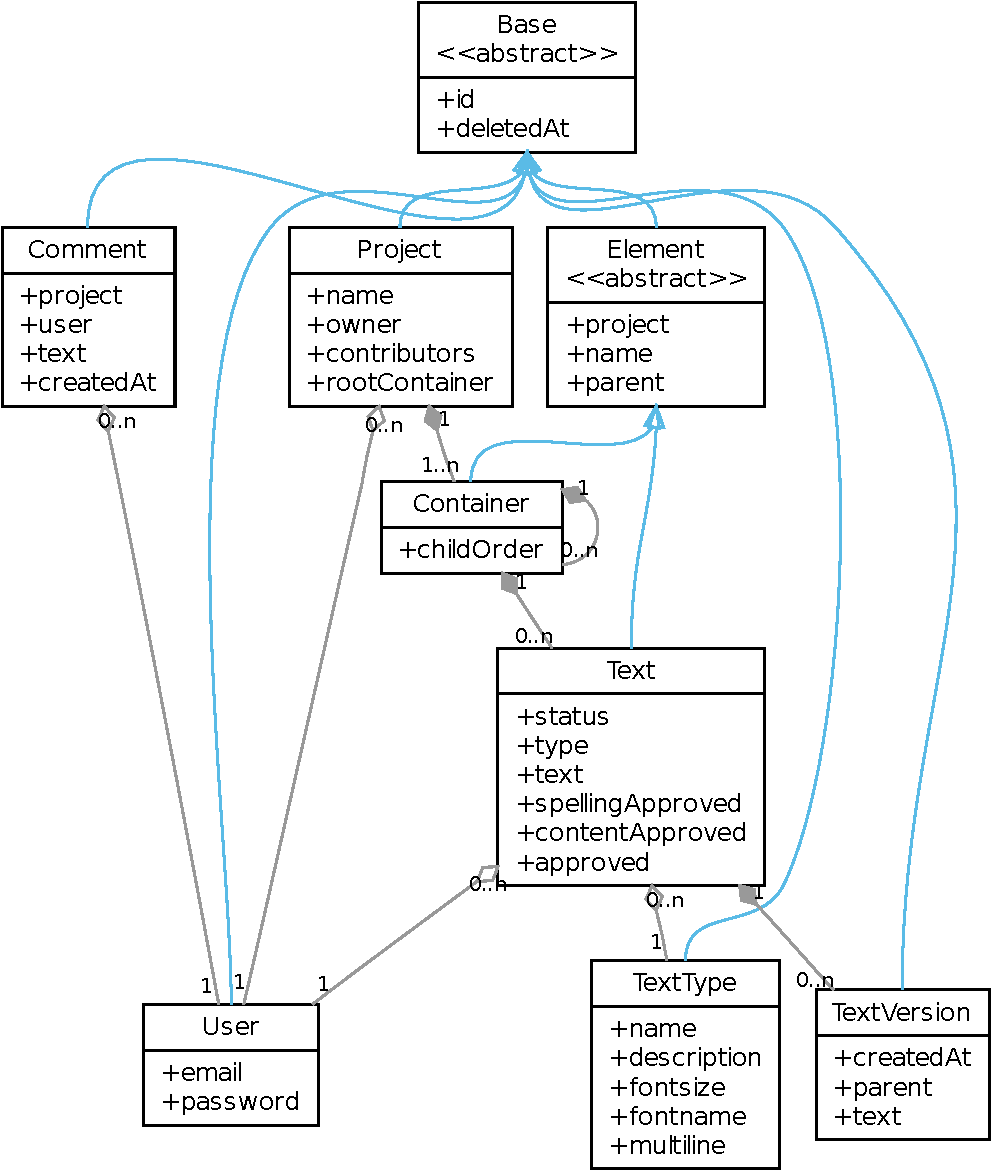
\includegraphics[width=0.65\textwidth]{media/prototyp-persistenz.pdf}
\captionof{figure}{Persistierte Objekte im Prototyp}\label{chart:prototype-persistenz}
\end{center}

Zum Persistieren der Daten kommt \trademark{MongoDB}\footnote{\url{http://www.mongodb.org/}}, eine No-SQL-Datenbank zum Einsatz, diese ermöglicht das unkomplizierte Speichern auch komplexer Dokumentenstrukturen. Die Wahl einer nicht-relationen Datenbank bietet den Vorteil, dass aufwändiges Zusammensetzen und Zerlegen von Dokumenten entfallen kann. In der Datenbank werden die in Abbildung \ref{chart:prototype-persistenz} gezeigten Domänenobjekte gespeichert. Dieses Modell ist deutlich einfacher als das in Abschnitt \ref{l:domänenmodell} · S.\pageref{l:domänenmodell} vorgestellte Domänenmodell, da im Prototyp nur wenige, entscheidende Funktionen implementiert wurden. Das Laden- und Speichern ist durch den Einsatz eines Object-Document-Mappers (ODM) für Doctrine 2 und MongoDB\footnote{\url{https://github.com/doctrine/mongodb-odm}} weitestgehend automatisiert. 

\subsubsection{Klassendiagramm}

\begin{center}
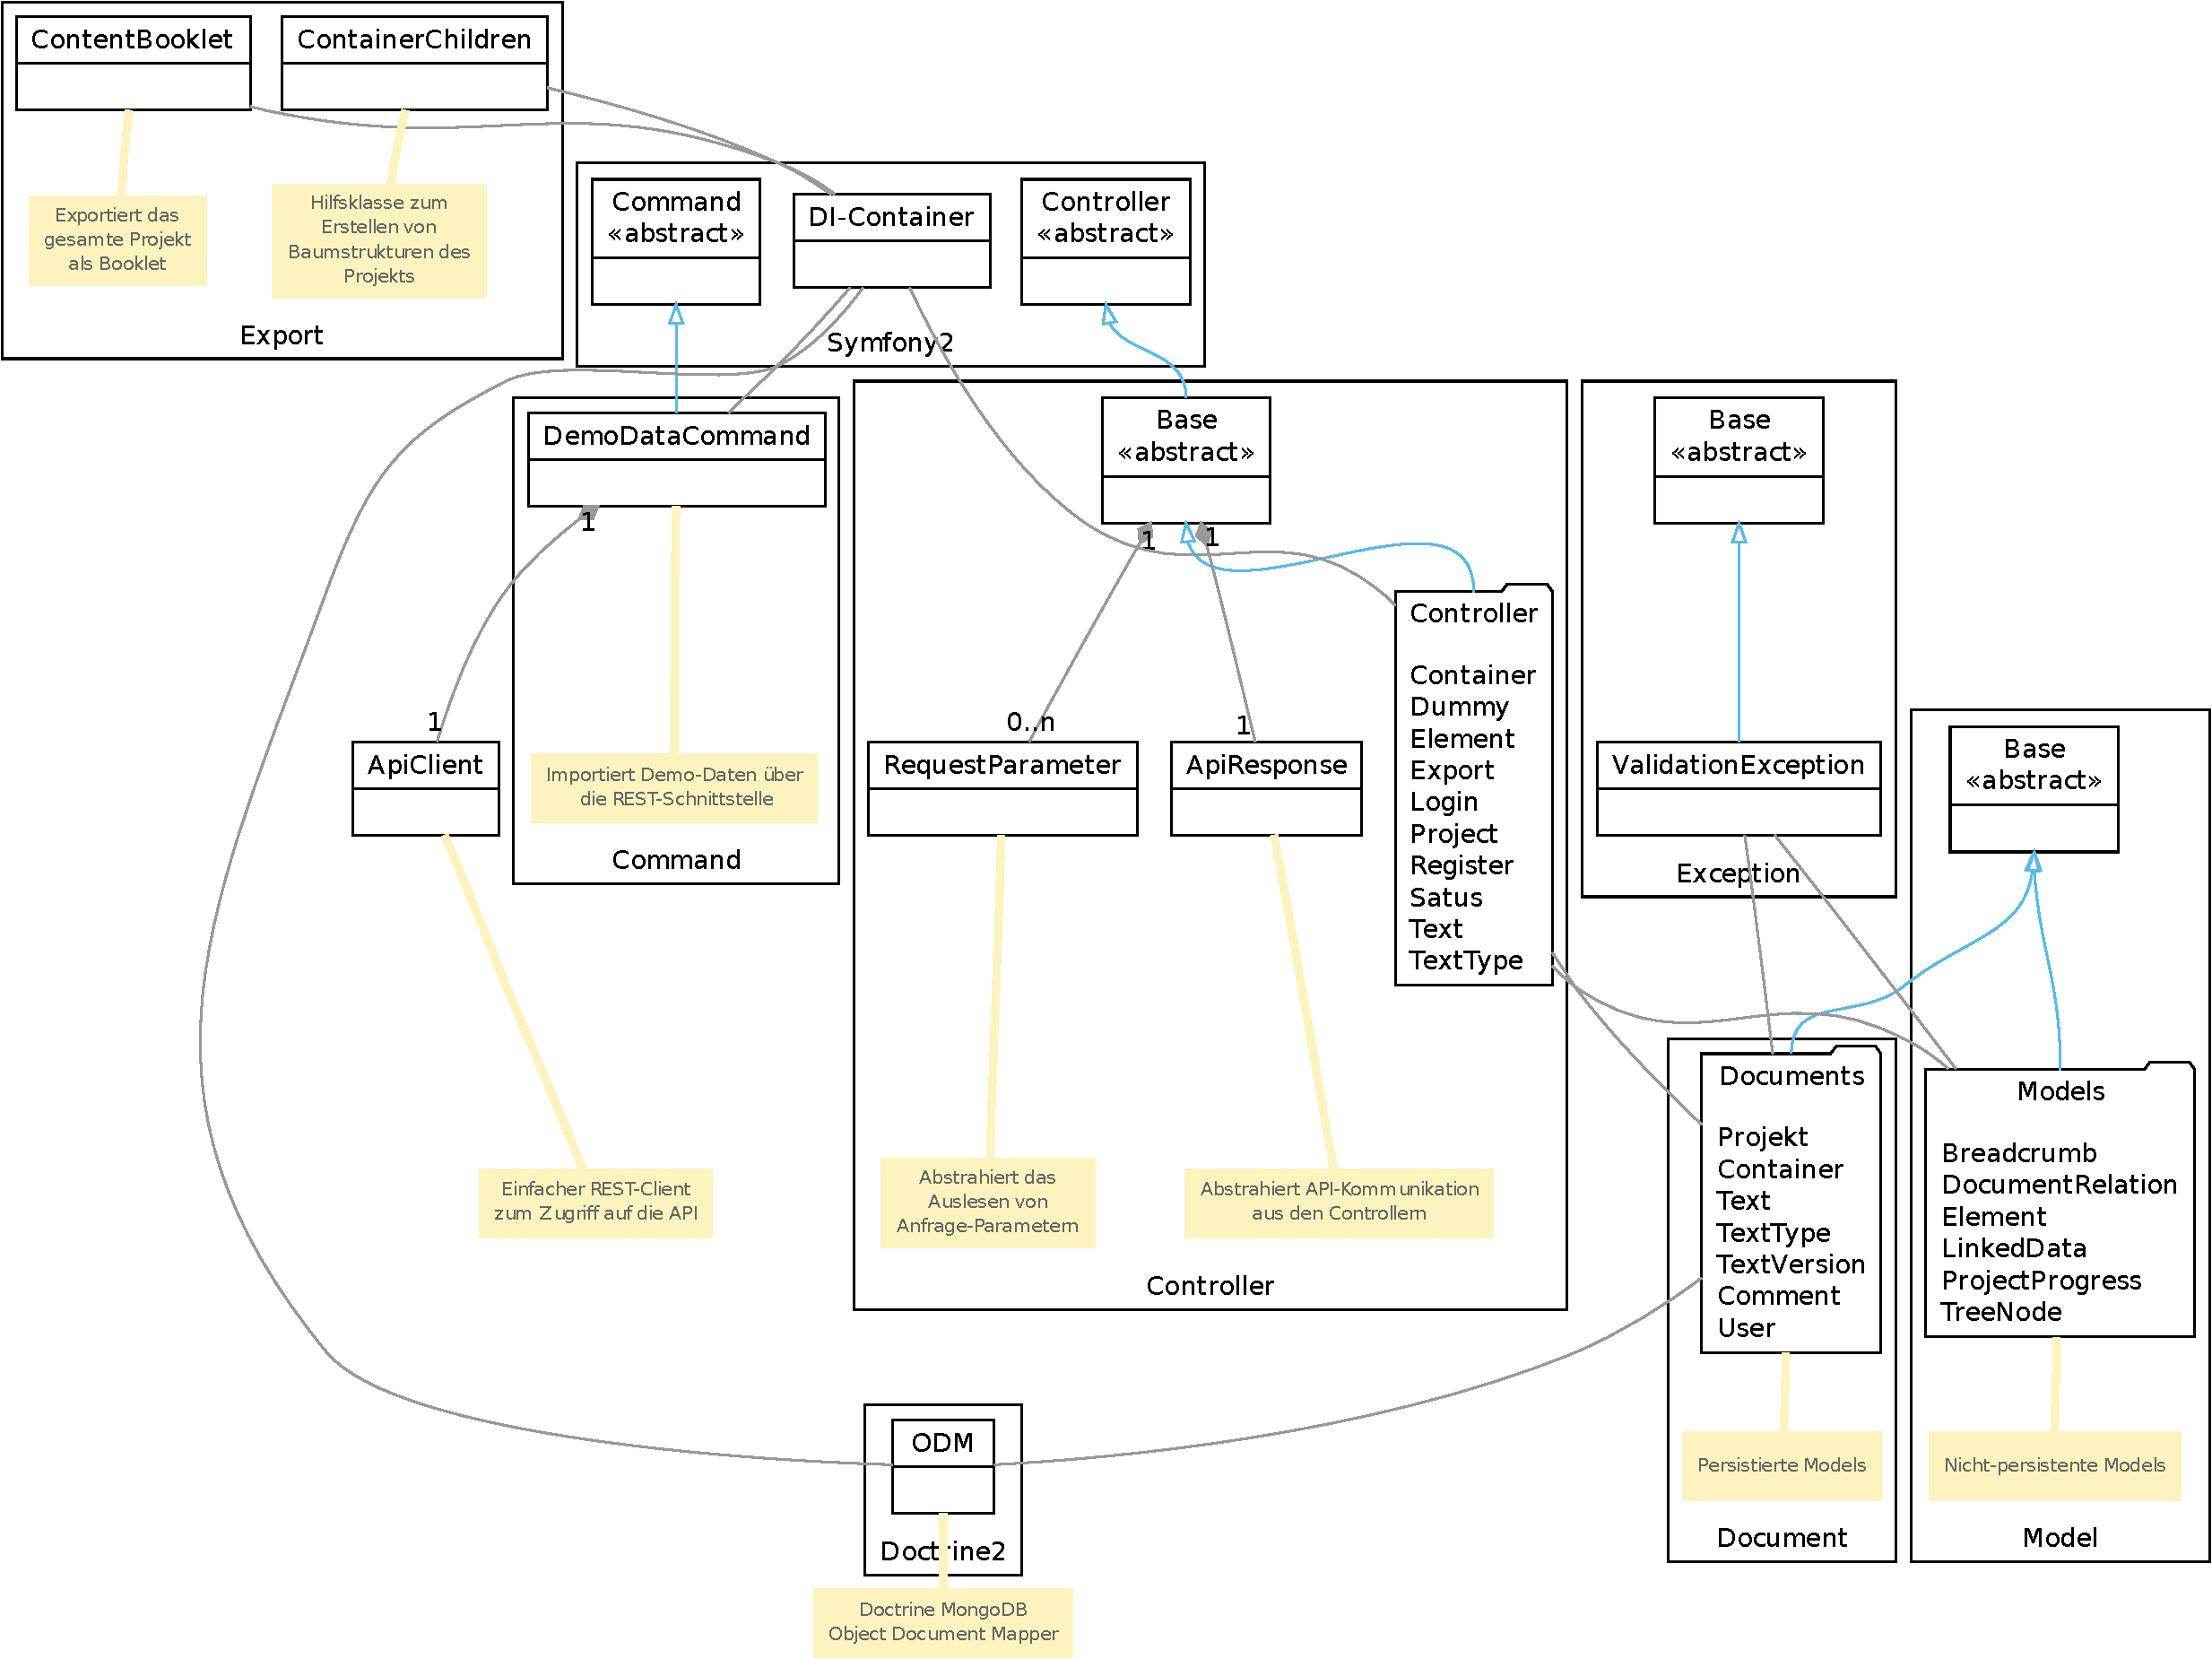
\includegraphics[width=\textwidth]{media/prototyp-klassendiagramm.pdf}
\captionof{figure}{Anwendungsserver-Klassendiagramm des Prototyps}\label{chart:prototyp-klassendiagramm}
\end{center}

Abbildung \ref{chart:prototyp-klassendiagramm} zeigt das Klassendiagramm der Implementierung des Prototyps. Zentrale Komponente ist der Dependency-Injection-Container des Symfony2-Frameworks, dieser instanziert je nach Pfad der Anfrage einen Controller und ruft dort die entsprechende Methode auf. Innerhalb der Controller steht der DI-Container zur Verfügung über den dann z.B. der ODM instanziert werden kann, um Daten aus der Datenbank zu laden. Der ODM verwendet zur Repräsentierung der Daten die Klassen des Packages \texttt{Documents}, die Controller können diese selber erzeugen, oder bekommen diese als Anfrage-Ergebnisse vom ODM übergeben.

Funktionen, die an mehreren Stellen, oder über unterschiedliche Arten verwendet werden, wurden in eigene Services ausgelagert (\texttt{ContentBooklet} und \texttt{ContainerChildren}). Diese werden zum einen innerhalb der Controller verwendet, können aber auch über das CLI gestartet werden. \trademark{Symfony2} stellt ein einfache Möglichkeit zum Erstellen vom Operationen über die Kommandozeile zur Verfügung. Im Prototyp wurde das Anlegen von Demo-Projekt-Daten mithilfe dieser Möglichkeit realisiert. Das \texttt{DemoDataCommand} wird von der Konsole aus gestartet und verwendet den \texttt{ApiClient}, um über HTTP mit der Schnittstelle des Anwendungsservers zu kommunizieren.

\secbar

Die Implementierung eines Prototyps dient zur Verifizierung des Entwurfs; im folgenden Abschnitt wird der Prototyp in einem realitätsnahen Szenario begutachtet.

\pagebreak

\subsection{Implementierter Workflow am Beispiel des Studiengangsflyers}

Die in den vorangegangenen Abschnitten vorgestellte Implementierung des Prototyps wird anhand eines realen Projekts auf ihre praxistauglichkeit hin überprüft. Es handelt sich dabei um die einmal im Jahr erscheinende Informationsbroschüre des Studienganges Medieninformatik an der Hochschule RheinMain. Die Broschüre zu Beginn des Wintersemesters 2011/2012 einen Umfang von 28 Seiten zuzüglich Titel und Rückseite. In ihr findet sich das Grußwort des Studiengangsleiters, eine Kurzinfo über den Studiengang, das Studienprogramm mit Informationen zum Verlauf des Studiums, ein Terminkalender, Informationen zu Einrichtungen des Fachbereiches, eine Liste mit Personen im Fachbereich, sowie eine Umgebungskarte und ein Gebäudeplan. Die Broschüre wird von den Mitarbeitern des Fachbereiches selber erstellt.

\bigskip

Mit dem Prototyp ist es möglich, den Flyer als Projekt anzulegen. Im nächsten Schritt wird die Struktur des Flyers festgelegt. Die Anwendung unterscheidet dazu zwischen Containern und Textbausteinen. Container sind rein strukturelle Elemente, die wiederum weitere Container und Textbausteine enthalten können. Für den Flyer bietet es sich an, einzelnen Kapitel (Titel, Vorwort, Kurzinfo, Termin \& Öffnungszeiten, Personen, Orientierung) als Container auf oberster Ebene anzulegen und daruntere jeweils weitere Unterteilungen nach Abschnitten vorzunehmen. Innerhalb dieser Abschnitte werden dann die einzelnen Textbausteine definiert. Zu den Textbausteinen können auch Zusatzinformationen zum Text-Typ (Schriftart, Schriftgröße, ein- oder mehrzeilig) hinterlegt werden. Die Elemente lassen sich mittels Drag\&Drop in der Reihenfolge anpassen.

Sobald die Bestandteile des Produkts angelegt wurden kann parallel bereits mit der Erstellung der Texte begonnen werden. Diese können in den jeweiligen Bausteinen je nach Typ als ein- oder mehrzeiliger Text hinterlegt werden. Änderungen an den Inhalten werden gespeichert und sind als Änderungsverlauf abrufbar. Über eine Kommentarfunktion ist der Austausch über die Texte innerhalb der Anwendung möglich. 

In der Ansicht zur Freigabe können die einzelnen Texte überprüft und abgenommen werden. Es wird zwischen den Stati für Rechtschreibung, Inhalt und der allgemeinen Freigabe unterschieden. Bei Statusänderungen wird automatisch ein Kommentar erzeugt, dass beim Ablehnen mit Zusatzinformationen durch den Benutzer versehen werden kann. Die einzelnen Stati werden aggregiert und als gesamt-Status für das gesamte Projekt angezeigt, sowie zur Übersicht und zum schnellen Zugriff in der Projektstruktur.

Als Beispiel für die Verwendung der Projektdaten in externen Systemen lässt sich das Projekt als \emph{Content-Booklet} im HTML- oder PDF-Format exportieren. Dieses Dokument enthält alle Information in strukturierter Form, so wie sie im System angelegt wurden und listet neben den Texten auch die jeweiligen Zusatzinformationen. Mit Hilfe des \emph{Content-Booklet} können Produzenten einfach mit der neuesten Version der Texte für das Produkt versorgt werden und es liefert einen Überblick über alle Bestandteile des Produkts. Ein Ausschnitt aus diesem Booklet findet sich in Anhang \ref{l:booklet} · S.\pageref{l:booklet}.

\secbar

Der Prototyp ist in der Lage, bereits mit diesem einfachen Funktionsumfang einen praktischen Mehrwehrt für ein Produkt wie den Studiengangsflyer zu bieten. Die Texte können gemeinsam und nachvollziehbar erfasst werden, der Export als \emph{Content-Booklet} kann verschiedene Mitarbeitern bei der Erstellung des fertigen Produkts konkrete Hilfestellung bieten.

\pagebreak

\subsection{Zusammenfassung}

In diesem Kapitel wurde das zentrale System der Anwendung, bestehend aus Server und browserbasierten GUI entworfen und beschrieben. Der Aufbau des Servers mithilfe einer lose gekoppelten Architektur ermöglich einfache Erweiterbarkeit und Wartung. Das browserbasierte GUI ist als JavaScript-MVC-Anwendung entworfen, die über eine REST-API mit dem Server kommuniziert. Die wichtigsten Ansichten des GUIs wurden mit Hilfe von Wireframes beschrieben. 

Der Entwurf wurde mithilfe einer prototypischen Implementierung, in der die wichtigsten Abläufe abgebildet werden, anhand eines realen Projekts überprüft. Dabei wurde gezeigt, dass sich die vorgeschlagenen Prinzipien, in der Darstellung wie in der Implementierung mit aktuell verfügbaren Technologien problemlos umsetzen lassen. Zudem wurde gezeigt, dass das Konzept der Trennung zwischen Anwendungsserver und GUI keine negativen Auswirkungen auf die Verwendbarkeit einer Anwendung hat. Für die Realisierung weiterer Funktionen im Sinne des Entwurfes sind keine Hindernisse aufgetreten.

Der in diesem Kapitel vorgestellte Entwurf liefert damit die Basis für die mögliche Entwicklung einer vollwertigen Lösung und bietet für einzelne Bestandteile bereits mögliche Technologieempfehlungen.

\secbar

Damit kann diese Bachelor-Thesis im nächsten und letzten Kapitel \ref{l:fazit} mit dem Fazit abgeschlossen werden.

\pagebreak
